\documentclass[12pt,leqno]{article}
%\documentclass[a4paper,12pt,twoside]{article}
%\documentclass[14pt,a4paper]{scrbook}

%\usepackage{float}
%\usepackage{listings}
%\usepackage{xkeyval}
%\usepackage{eucal}
%\usepackage{mathrsfs}
%\usepackage{theorem}
%\usepackage{pifont}
% \usepackage{bibtopic,wrapfig}
%\usepackage{bbding}
%\usepackage{fancyhdr}
%\usepackage{verbatim}
%\usepackage{bidi}

% User packages
%%%%%%%%%%%%%%%%%%%%%%%%%%%%%%%%
\usepackage{amsmath,amsfonts,amssymb}
% \usepackage{graphicx}
% \usepackage{pgfplots}
%\usepackage{color} %red, green, blue, yellow, cyan, magenta, black, white
% \definecolor{mygreen}{RGB}{28,172,0} % color values Red, Green, Blue
% \definecolor{mylilas}{RGB}{170,55,241}
% \usepackage{graphicx}
% \usepackage{epstopdf}
% \usepackage{epsfig}
\usepackage[hyperindex,colorlinks]{hyperref}
%\usepackage[colorlinks=true, bookmarks=true]{hyperref}
\usepackage{subcaption}
\usepackage{mathtools}
\usepackage{pdfpages}
\linespread{1.4}
\usepackage[lmargin=1in,rmargin=1in,tmargin=1in]{geometry}

\usepackage{fontspec}
\usepackage{polyglossia}
\setdefaultlanguage{hebrew}
\setotherlanguages{english}
\newfontfamily\hebrewfont[Script=Hebrew]{David}
% \usepackage{bidi}


%\rhead{\thepage}
%\lfoot{\small \copyright\;\;\; שירה בר-דב, אורט בראודה}
%\rfoot{\thepage}
%\cfoot{}
%\renewcommand{\headrulewidth}{0.4pt}
%\renewcommand{\footrulewidth}{0.4pt}
%\DeclareGraphicsExtensions{.pdf,.png,.jpg}
%\let\arref\ref
%\renewcommand{\ref}[1]{\I{\arref{#1}}}




%\rhead{\thepage}
%\lfoot{\small \copyright\;\;\; שירה בר-דב, אורט בראודה}
%\rfoot{\thepage}
%\cfoot{}
%\renewcommand{\headrulewidth}{0.4pt}
%\renewcommand{\footrulewidth}{0.4pt}
%\DeclareGraphicsExtensions{.pdf,.png,.jpg}
%\let\arref\ref
%\renewcommand{\ref}[1]{\I{\arref{#1}}}

% \setlength{\parskip}{4pt plus 2pt} \setlength{\parindent}{0pt}
% \setlength{\oddsidemargin}{0pt} \setlength{\evensidemargin}{0pt}

% User defined macros
%%%%%%%%%%%%%%%%%%%%%%%%%%%%%%%%

\newtheorem{definition}{הגדרה}[section]
\newtheorem{theorem}{משפט}[section]
\newtheorem{proposition}{טענה}[section]
\newtheorem{conjecture}{השערה}[section]
\newtheorem{corollary}{מסקנה}[section]
\newtheorem{lemma}{למה}[section]
\newtheorem{example}{דוגמה}[section]
\newtheorem{comm}{הערה}[section]

\newcommand{\sumi}[1]{\sum_{#1=1}^n}
\newcommand{\Zn}{{\mathbb{Z}_2}^n}

%\numberwithin{equation}{section}

%\documentclass{amsart}
%%\usepackage[active]{srcltx} % SRC Specials for DVI Searching
%\usepackage {epsfig}
%% THEOREM Environments ---------------------------------------------------
% \newtheorem{thm}{Theorem}
% \newtheorem{cor}[thm]{Corollary}
% \newtheorem{lemma}[thm]{Lemma}
% \newtheorem{prop}[thm]{Proposition}
% \newtheorem{theorem}[thm]{Theorem}
% \theoremstyle{definition}
% \newtheorem{defn}[thm]{Definition}
% \theoremstyle{remark}
% \newtheorem{rem}[thm]{Remark}
%% MATH -------------------------------------------------------------------
%%%% ----------------------------------------------------------------------
%\setlength{\textheight}{43pc} \setlength{\textwidth}{28pc}
%

% User defined macros
%%%%%%%%%%%%%%%%%%%%%%%%%%%%%%%%


\begin{document}

\begin{titlepage}
\newcommand{\HRule}{\rule{\linewidth}{0.5mm}} % Defines a new command for the horizontal lines, change thickness here

\center % Center everything on the page

%----------------------------------------------------------------------------------------
%   HEADING SECTIONS
%----------------------------------------------------------------------------------------

{\LARGE 
המחלקה למתמטיקה שימושית
 % Major heading such as course name
}
\vspace{20pt}

%----------------------------------------------------------------------------------------
%   TITLE SECTION
%----------------------------------------------------------------------------------------

\HRule \\[0.4cm]
{ \huge \bfseries
חקירת משחק האורות
% Title of your document
 } \\[0.4cm] 
\HRule \\[1.5cm]

%----------------------------------------------------------------------------------------
%   AUTHOR SECTION
%----------------------------------------------------------------------------------------
\hspace{50pt}  
\begin{minipage}{0.4\textwidth}
    \begin{flushright} \large
    מאת:
    \\
    ולדיסלב ברקנס
    \end{flushright}
\end{minipage}
    ~
\begin{minipage}{0.4\textwidth}
    \begin{flushright} \large
    מנחה:
    \\
    אלכס גולוורד 
    % Supervisor's Name
    \end{flushright}
\end{minipage}\\[2cm]

%----------------------------------------------------------------------------------------
%   DATE SECTION
%----------------------------------------------------------------------------------------

{\large \today} \\[2cm] % Date, change the \today to a set date if you want to be precise
%----------------------------------------------------------------------------------------
%   LOGO SECTION
%----------------------------------------------------------------------------------------
\begin{figure}
	\begin{center}
		{\includegraphics[scale=0.3]{images/Braude_Logo.jpg}}
	\end{center}
%	\caption{הפונקציה $\arctan(x)$ - באדום, וסכום שלושת האיברים הראשונים של טור טיילור שלה - בכחול}
%	\label{atan}
\end{figure}

%\includegraphics[scale=0.3]{Braude_Logo}\\[1cm] % Include a department/university logo - this will require the graphics package
%----------------------------------------------------------------------------------------

\vfill % Fill the rest of the page with whitespace

\end{titlepage}
%----------------------------------------------------------------------------------------
%   תוכן עניינים
%----------------------------------------------------------------------------------------
\tableofcontents

\newpage
%--------------------------------------------------------------------------------------
%   הקדמה
%----------------------------------------------------------------------------------------
\section{הקדמה}
עבודה זה הינה עבדות סוף של סטודנט במחלקה למתמטיקה שימושית.
עבודה זה 
מבוססת על משחק האורות 
ונבנתה 
על  גבי שאלות שנשאלו במהלך חקירת המשחק.
חיפוש פתרונות הוביל למחקר ותוצאות מעניינות 
שלא ברורות מעליהן.

השאלות לדוגמה שעלו בעבודה הן שיטות למציאת פתרון למשחק.
נציג שתי שיטות, שבדיעבד נראו שונות אבל הצלחנו להראות את הקשר בשתי השיטות.

בנוסף 
לאחר שנמצא אלגוריתם שפותר את המשחק שמנו לב לתופעה מעניינת  כאשר המשחק האורות
מתחיל כאשר כל הנורות דלוקות אז קיים לפחות פתרון אחד,
תופעה מעניינת שכזה העסיקה רבות את פרויקט זה ומצאנו הוכחה מדוע תופעה זה מתקיימת.

דבר מרכזי נוסף שעסקנו בו הוא בחיפוש סוג מסוים של פתרונות, פתרונות מינמלי שנגדיר בעבודה. 
סוג הפתרונות שכזה כל כך לא נפוץ שהצלחנו להוכיח את כל המקרים 
בהם אתכן פתרון שכזה.

עבודה סוף זה הייתה מהנה עבורי אני מודה למחלקה
למתמטיקה שימושית
\\
במיוחד לאלכס גולוורד על הזדמנות לעשות 
עבודה מרתקת שכזה.

תודה רבה

\newpage

\section{תאור של המשחק}
משחק האורות או 
\textenglish{Lights Out}
בלועזית,
זהו משחק על לוח משבצות מלבני.
כל משבצת יכולה להיות באחד משני מצבים, נקרא להם דלוק וכבוי.
כאשר משתמשים בשמות האלה מתכוונים שבכל משבצת יש נורה והיא יכולה להיות דולקת או כבויה. במצב התחלתי כל הנורות כבויות.
יש לנו לוח בקרה שמאפשר בכל שלב של המשחק ללחוץ על משבצת ולשנות את מצב הנורה: אם היא דולקת לכבות אותה ואם היא כבויה להדליק אותה.
לוח בקרה בנוי כך שכאשר מתבצעת לחיצה על משבצת אז מצב של נורה משתנה ומשתנה גם מצב של נורות סמוכות לה.
שתי נורות נקראות סמוכות אם הן נמצאות במשבצות בעלות צלע משוטפת.
המטרה של המשחק היא לעבור ממצב התחלתי למצב בו כל הנורות יהיו דולקות. 

\begin{comm}
    בחירת מצב התחלתי להיות דלוק או כבוי אינה תשנה את המשחק.
\end{comm}
הערה מדגישה כי כל המטרה של המשחק היא לעבור ממצב מסוים בו נמצאים כל הנורות למצב אחר.
איך ניקרא למצב או איך שהוא יראה בפועל לא משנה את אופי המשחק אבל מה שחשוב שיש שני מצבים התחלתי וסופי.

\subsection{תאור גרפי של המשחק}
נתאר את המשחק באיור כאשר
המצב התחלתי של משחק שכל נורות
צהובות, ומצב הסופי היה שכל נורות שחורות.
נסמן את המשבצת שנלחצה בגבולות ירוקים.

\begin{figure}[ht]
    \caption{הסבר שינוי מצב הלוח לאחר לחיצה}
    \centering
    \label{fig: explain game}
    \begin{subfigure}{.3\textwidth}
        % \unsethebrew
        \caption{לוח במצב התחלתי}
        \label{subfig: explain game, start}
        \centering
        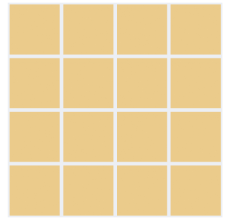
\includegraphics[scale=0.67]{images/4x4_start_board.PNG}
        % \sethebrew
    \end{subfigure}%
    \begin{subfigure}{.3\textwidth}
        % \unsethebrew
        \caption{לוח לאחר לחיצה בודדת}
        \label{subfig: explain game, move}
        \centering
        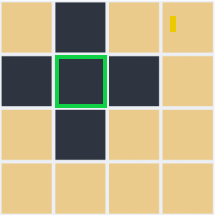
\includegraphics[scale=0.67]{images/4x4_press.PNG}
        % \sethebrew
    \end{subfigure}%
    \begin{subfigure}{.3\textwidth}
        % \unsethebrew
        \caption{לוח לאחר שני לחיצות}
        \label{subfig: explain game, next move}
        \centering
        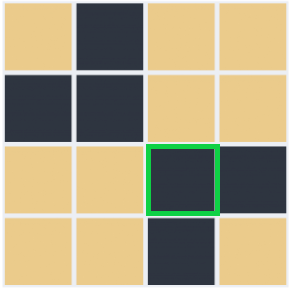
\includegraphics[scale=0.49]{images/4x4_next_press.PNG}
        % \sethebrew
    \end{subfigure}%
\end{figure}
פירוט:
נבחין כי המשחק 
על לוח
$4 \times 4$
המצב התחלתי מתואר
באיור
\ref{subfig: explain game, start}
במצב של הלוח
כל הנורות צהובות.
לאחר ביצוע לחיצה על משבצת שמסומנת בירוק נעבור ללוח שמתואר באיור 
\ref{subfig: explain game, move}.
נתאר לחיצה נוספת באיור 
\ref{subfig: explain game, next move}.

אחרי שהסברנו על כללי משחק והצגנו הדגמה קטנה הדרך הטובה ביותר לוודא הבנה היא בלשחק,
כפי שנאמר "עדיף לראות פעם אחת, מאשר לשמוע מאה פעמים"
או במקרה שלנו לשחק.
את המשחק אפשר לשחק בקישור הבאה:
\url{https://www.geogebra.org/m/JexnDJpt#chapter/301822}.

אתגר שכל שחקן חווה היא 
שאין אסטרטגיה גלויה למציאת פתרון, בפועל מנסים להגיע למצבים ידועים
שמהם אתה מכיר את איך לפתרו את המשחק. 
לכן כל פעם שמנסים משחק על לוח בממדים חדשים, חוויה
המשחק מתחדשת כאילו ולא שיחקת במשחק מעולם.

\subsection{סוגיות בהן נעסוק בפרויקט}
\begin{enumerate}
	\item 
	תיאור ודיון בשני אלגוריתמים למציאת פתרון המשחק.
	\item 
	הוכחות לקיום פתרון המשחק לכל לוח
	$m\times n$.
	\item 
	הרחבה של משחק מלוח משבצות למשחק על גרף.
	\item 
    חיפוש לוחות של משחקים בהם מתקיים פתרון כזה שנורות שינו את מצבן רק פעם אחת בלבד.
    \item 
    נתן התייחסות למספר הפתרון האפשריים בלוח ונדבר על חסם מספר הפתרונות על לוח בממדים כלשהם
\end{enumerate}

קיימים המון שאלות שקשורות למשחק וננסה בפרויקט זה להציג פתרון לחלקם.
נרצה בפרויקט זה להציג תופעות מעניינות במשחק, ולהראות
שהמשחק אינו רק מהנה עלה גם אתגר מתמטי לא קטן.

\subsection{תיאור משחק על גרף}
אחרי שכללי המשחק על לוח הובנו אפשר לנסות להכליל את המשחק כמשחק על גרף.
נזכיר שגרף זה מבנה המכיל קשתות וצמתים, קשתות מוגדרות כצירוף סדור של שני צמתים.
כדי לתאר את משחק האורות על גרף נשתמש באותם כללים שהגדרנו.
הבדל הוא שבמשחק על גרף הצמתים מקבלים את התפקיד של הלחצנים, לאומת אותם המשבצות שהיו במשחק על לוח.
נזכיר שכל לחיצה על צומת הופכת את המצב של אותה הצומת והשכנים שלה,
כאשר המשחק הוא על גרף נומר שצמתים שכנים אם קיימת
קשת שמחברת ביניהם.
נציין כי כאשר כל צומת יכולה להיות בשתי מצבים,
דלוקה או כבויה.
המטרה במשחק לעבור מגרף הצמתים במצב מסוים נגיד דלוק למצב אחר כבוי.

\begin{figure}[ht]
    \caption{משחק על גרף לדוגמה}
    \label{fig: start game in graph}
    \begin{subfigure}{.5\textwidth}
        % \unsethebrew
        \centering
        \caption{מצב התחלתי}
        \label{subfig: graph game start}
        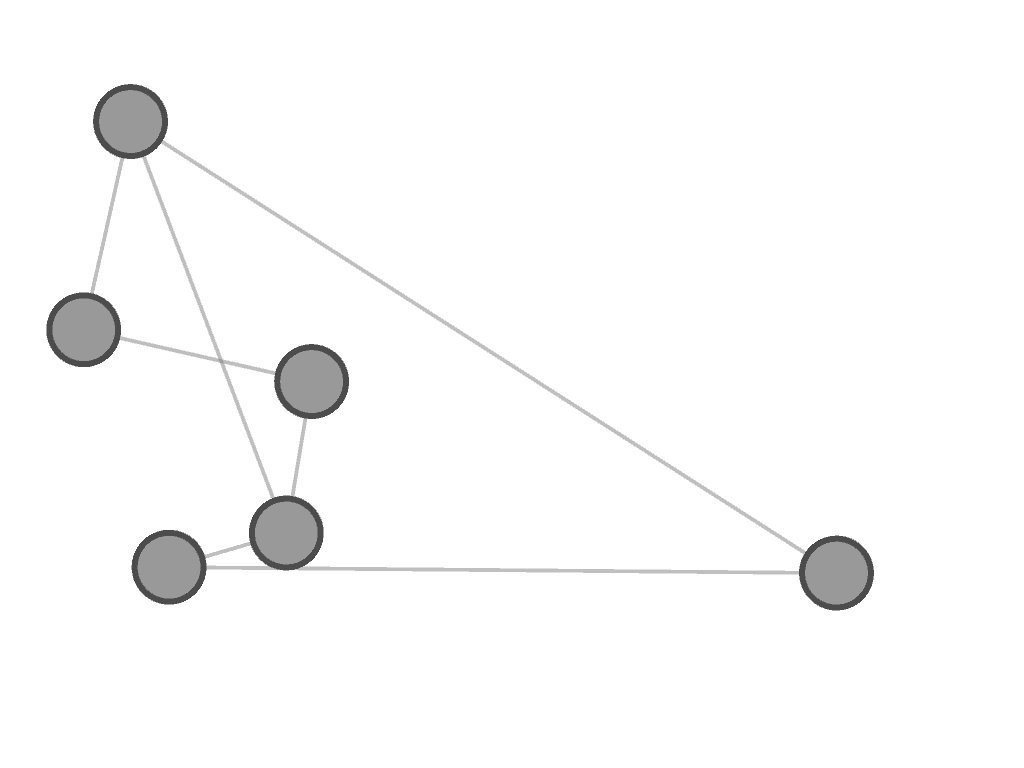
\includegraphics[scale=0.7]{images/graph_start_board.png}
        % \sethebrew
    \end{subfigure}%
    \begin{subfigure}{.5\textwidth}
        % \unsethebrew
        \centering
        \caption{לחיצה על משבצת מסומנת}
        \label{subfig: graph game move}
        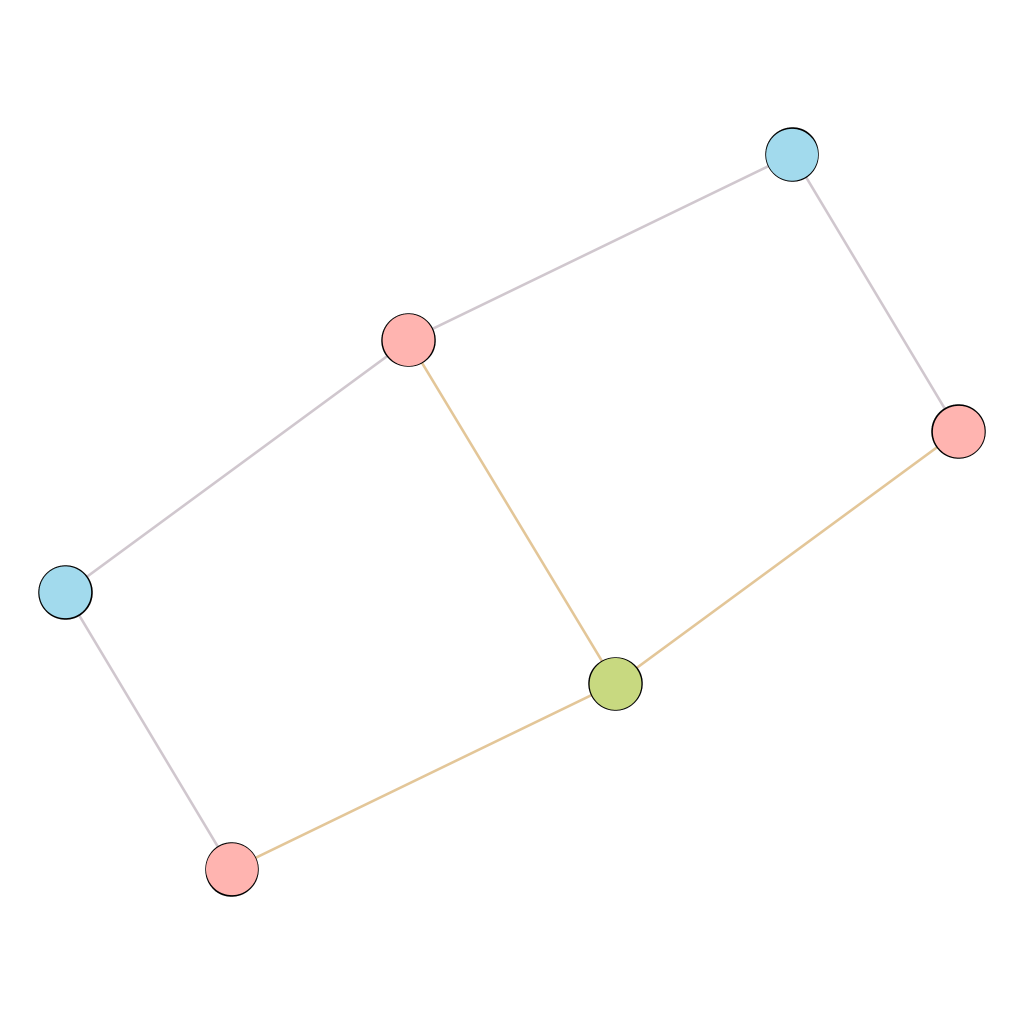
\includegraphics[scale=0.7]{images/graph_press.png}
        % \sethebrew
    \end{subfigure}%
\end{figure}

נמחיש זאת על דוגמה שבאיור
\ref{fig: start game in graph}
כאשר הגרף התחלתי
\ref{subfig: graph game start}
ניתן לראות
$6$
קודקודיים
צבועים באפור כלומר כבויים ומטרה של המשחק להדליק את כל הצמתים כלומר לצבוע את כולם בצהוב.
בשלב 
\ref{subfig: graph game move}
צומת שנלחצה נצבע בירוקה היא ושכניה נדלקות ונצבעות בצהוב.

\begin{comm}
    בפועל צומת ירוקה גם נצבעת לצהוב צביעה לירוק נועדה להדגשה על מי בוצע הלחיצה.
\end{comm}

\subsection{תרגום משחק על לוח למשחק על גרף}
לאחר שתיארנו כיצד לשחק את המשחק על גרף ניתן לומר ששחק על לוח
הוא סוג של משחק על גרף
כלומר, כל משחק 
לוח ניתן לתאר בעזרת משחק על גרף.
נרצה בתת פרק לחדד זאת.

כדי לתאר את הלוח על על משחק על גרף נשתמש בשני הכללים הבאים:
\begin{enumerate}
    \item 
    כל משבצת על משחק לוח נהפוך לצומת.
    \item 
    כל זוג משבצות סמוכות על לוח נחבר את הצמתים בצלע
\end{enumerate}

נמחיש זאת על דוגמה, ניקח לוח למשל
$2 \times 3$
נמספר את המשבצות כמו באיור
\ref{2x3_board}.
הגרף שנקבל עבור לוח באיור
\ref{2x3_board}
מתואר באיור
\ref{2x3_graph}

\begin{figure}[ht]
    \caption{
        דוגמה
        למשחק על לוח שתורגם למשחק על גרף
        }
    % \label{fig: start game in graph}
    \begin{subfigure}{.5\textwidth}
        \caption{
            משחק על לוח
            $2 \times 3$
            שמשבצותיו
            ממוספר
        }
        \label{2x3_board}
        % \unsethebrew
        \centering
        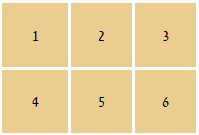
\includegraphics[scale=0.9]{images/2x3_board.PNG}
        % \sethebrew
    \end{subfigure}%
    \begin{subfigure}{.5\textwidth}
        \caption{
            משחק על גרף
            שתורגם מלוח
            $2 \times 3$
        }
        % \unsethebrew
        \centering
        \label{2x3_graph}
        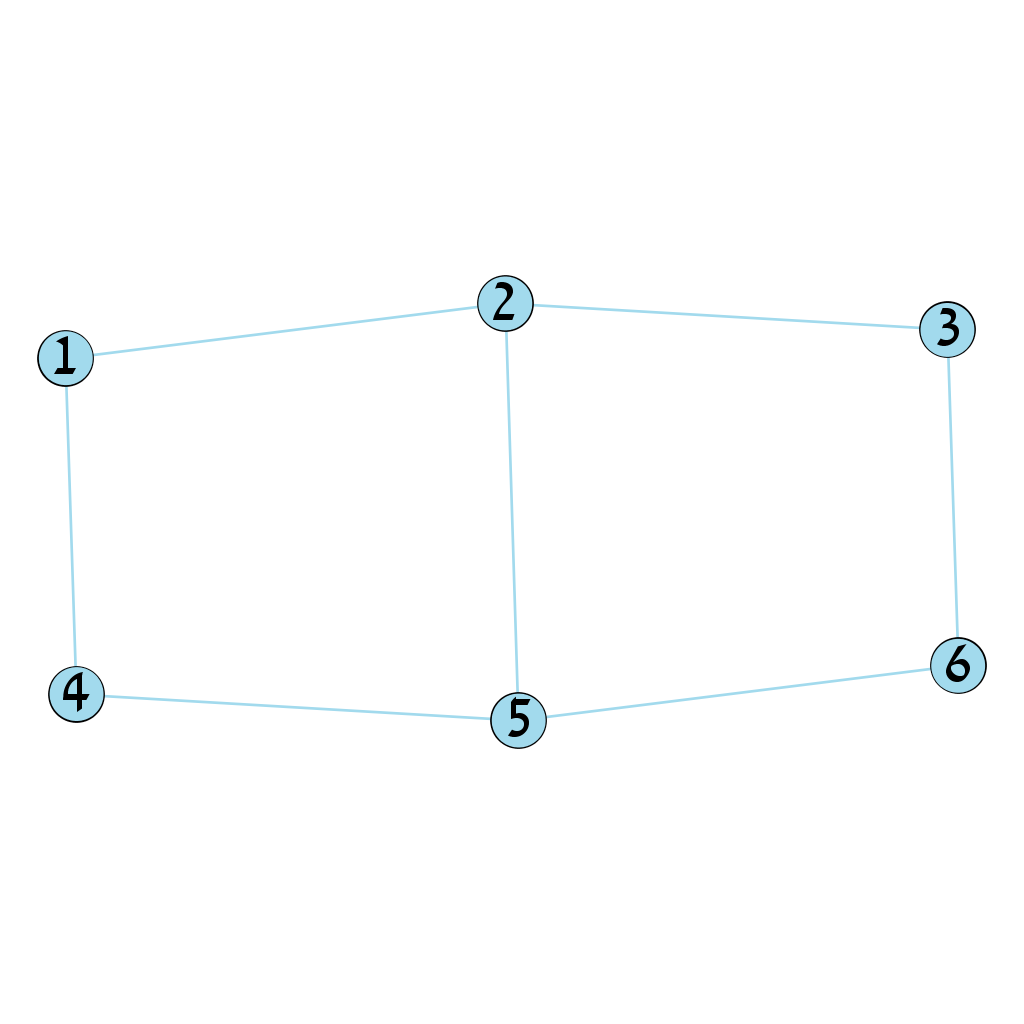
\includegraphics[scale=1]{images/2x3_graph.png}
        % \sethebrew
    \end{subfigure}%
\end{figure}


\begin{comm}
    קיימים הרבה משחקים שמתוארים על גרף אבל לא ניתן לתאר אותם על לוח
    לדוגמה,
    גרף בו יש צומת אם יותר מ
    $4$
    שכנים לא ניתן לתאר לוח שכזה כיוון שלכל משבצת על לוח
    יש לכל יותר 
    $4$
    משבצות סמוכות.
\end{comm}

\begin{comm}
    בעזרת שיטה שתיארנו אפשר להפוך כל משחק לוח למשחק על גרף, אבל להפך הוא לא נכון 
    כלומר לא כל משחק על גרף אפשר להפוך למשחק על לוח.
\end{comm}

בגלל שכל משחק לוח ניתן לתאר אותו כמשחק על גרף לכן המשפטים המרכזיים ננסה לנסח על משחקים על גרף כי אז הם היו נכונים
גם על משחקים על לוח.


\newpage

\section{ אלגוריתם למציאת פתרון}

לפני שנציג את שיטות למציאת פתרון, נרצה להמחיש את 
האתגר במשחק על ידי הצגה כמה תופעות שקוראות במשחק.

באיור
\ref{fig:sol_3_4_5}
מוצגים כמה פתרונות אפשריים ללוחות שונים, כאשר לחיצה על הלחצנים ירוקים
בסדר כלשהו תוביל לפתרון המשחק.
אפשר לראות שכמות הלחיצות שצריך לפתרון 
על לוח 
$4 \times 4$
דורשת פחות לחיצות מהלוח 
$3 \time 3$.
ההנחה הגיונית 
שאפשר היה לחשוב היא שככל שהלוח גדול יותר נדרש 
יותר לחיצות 
כדי להגיע לפתרון,
אבל כפי שרואים 
באיור 
\ref{fig:sol_3_4_5}
זה לא נכון.

תופעה נוסף שקוראת במשחק היא שכמות הפתרונות משתנה.
עבור לוח 
$3 \times 3$
קיים פתרון יחיד,
אבל ללוח 
$4 \times 4$
קיים
$16$
פתרונות.
בהפתעה רבה ללוח 
$5 \times 5$
יש רק 
$4$.
עובדה זה שללוח 
$5 \times 5$
יש פחות פתרונות מלוח 
$4 \times 4$
מפתיע כי אפשר היה לצפות שלוח יותר גדול אז כמות הפתרונות תגדל.

אפשר לחדד את חוסר הבנה לכמות הפתרונות אם ניקח לדוגמה לוחות ריבועים כלומר
$n \times n$
כמות הפתרונות כל כך לא צפויה
שאם נשאל את עצמנו, מה הלוח אם הכי הרבה פתרונות וכמה פתרונות יש ללוח כאשר
\\
$n \in [1,20]$?
נקבל שמספר הפתרונות הגדול ביותר הוא על לוח
$n = 19$ 
ומספר פתרונות 
$65536$.
בנוסף
$n = 19$ 
הוא הלוח היחיד ב
$n \in [1,20]$
שמקבל
כמות הפתרונות שכזה.
לאומת זאת
מספר הפתרונות השני הגדול ביותר הוא רק
$256$
ומתקיים ל
$n \in \{9, 16 \}$.

\begin{figure}[ht]
    \caption{פתרונות של משחק על לוחות שונים}
    % \unsethebrew
    \label{fig:sol_3_4_5}
    \centering
    \begin{subfigure}[b]{.25\linewidth}
    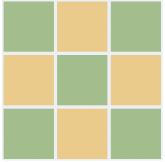
\includegraphics[width=0.95\linewidth]{images/3x3_sol.PNG}
    \end{subfigure}
    \begin{subfigure}[b]{.25\linewidth}
    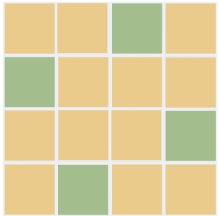
\includegraphics[width=0.97\linewidth]{images/4x4_sol.PNG}
    \end{subfigure}
    \begin{subfigure}[b]{.25\linewidth}
    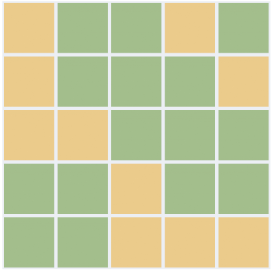
\includegraphics[width=0.95\linewidth]{images/5x5_sol.PNG}
    \end{subfigure}
\end{figure}

שתי השיטות למציאת פתרון שנציג בעבודה היו מבוססות
על מידול הבעיה לשדה לינארי ולמערכת משוואות שפתרון שלה יוביל לפתרון של המשחק עצמו.
אתכן ויש כמה דרכים להגיע לאותו מודלו לינארי שנציע, נציג בעובדה זה שני דרכים.
כשנתאר את שתי שיטות הן יראו שונות בתכלית אבל,
היופי הוא שאפשר להראות ששתי השיטות מובילות לאותה מערכת משוואות
כלומר צורת הפתרון המתוחכמת יותר נעזרת בצורה של הלוח כדי לפתור ביעילות גבוה יותר את הבעיה.

\subsection{שיטת פתרון ראשונה בעזרת מטריצת שכנויות}
כדי למדל את הבעיה על שדה לינארי נזכר בייצוג גרפי שאומר כי לחיצה על צומת משנה את הצומת ושכניה 
אם נסמן את צמתים ב
$n_i$
אז משלב זה נתאר את המשחק בצורה נוחה יותר לתיאור אלגברי.
\begin{enumerate}
    \item 
    כל צומת יכול להיות בשתי מצבים,
    את המצבים נסמן,
    ${0,1}$
    \item 
    מצב של צומת 
    $i$
    נסמן ב
    $n_i$.
    \item 
    המצב התחלתי של משחק על גרף הוא שכל צמתים אם הערך התחלתי
    שהוא 
    $0$.
    \item 
    מצב סופי של משחק
    על גרף הוא שכל צמתים 
    אם הערך הסופי
    שהוא
    $1$.
\end{enumerate}

\begin{comm}
    \label{comm: sum as press operator on board}
    פעולת לחיצה על לחצן משנה 
    את מצב מנורה,
    שינוי מצב מנורה ניתן 
    בעזרת חיבור 
    בשדה 
    $\mathbb{Z}_2$
    עם הערך 
    $1$.
    אם מצב צומת במצב התחלתי לאחר לחיצה 
    תעבור למצב 
    סופי,
    $0+1=1$.
    אם מצב צומת במצב הסופי לאחר לחיצה 
    תעבור למצב 
    התחלתי,
    $1+1=0$.
\end{comm}
תיאור של משחק שכזה מאפשרת לנו
לתאר המשחק בצורה וקוטרית.
אם ניקח לדוגמה
משחק בגודל
$2 \times 2$
נמספר את 
שורות ואז עמודות מלמעלה למטה כמו שמתואר באיור
\ref{fig:numbering_board_2x2}.
נוכל לתאר את הלוח 
שכזה במצבו התחלתי כמטריצה
\[\begin{bmatrix}
0 & 0 \\
0 & 0 
\end{bmatrix}\]
ואם נרצה לתאר את לוח ממצב התחלתי לאחר לחיצה על משבצת 
$1$.
\[ 
    \begin{bmatrix}
    0 & 0 \\
    0 & 0 
    \end{bmatrix} \stackrel{n_1}{\longrightarrow}
    \begin{bmatrix}
    1 & 1 \\
    1 & 0 
    \end{bmatrix}
 \]
 כפי שתיארנו 
 בהערה 
 \ref{comm: sum as press operator on board}
 אפשר לתאר שינוי מצב הנורה על ידי חיבור 
 עם אחד.
\[
    \begin{bmatrix}
    0 & 0 \\
    0 & 0 
    \end{bmatrix} + 
    \begin{bmatrix}
    1 & 1 \\
    1 & 0 
    \end{bmatrix}=
    \begin{bmatrix}
    1 & 1 \\
    1 & 0 
    \end{bmatrix} 
\]  
 אם נציג כל מטריצה ע"י ווקטור קואורדינטות בסיס סטנדרטי של מרחב מטריצות אז נוכל לרשום את השוויון הנ"ל גם כך
 \[ 
    \begin{bmatrix} 
    0 \\ 0 \\ 0 \\ 0
    \end{bmatrix} +  \begin{bmatrix} 
    1 \\ 1 \\ 1 \\ 0
    \end{bmatrix} =  \begin{bmatrix} 
    1 \\ 1 \\ 1 \\ 0
    \end{bmatrix}  
 \]
וקטור שחיברנו עם מצב הלוח התחלתי הוא וקטור שמתאר את הלחיצה ונקראה לו בעבודה זה וקטור שינוי.
 \begin{definition}
    תהי 
    משחק על גרף בעל
    $n$
    צמתים
    ממספרים מ
    $1$
    עד
    $n$,
    וקטור שינוי
    $t_i$
    של צומת  
    $i$
    הוא 
    וקטור 
    שייך 
    $\Zn$,
    שאם תחבר אותו אם מצב הלוח הנוכחי 
    התוצאה המתקבלת תהיה מצב הלוח 
    לאחר לחיצה על צומת 
    $i$.
\end{definition}
כדי לבנות וקטור שינו 
של 
צומת 
$i$
נשים ערך 
$1$
בכל אינדקסים 
בהם האינדקס שווה 
למספור 
של 
צומת 
שכנה
לצומת
$i$
ובאינדקס של צומת עצמה
כלומר,
באינדקס 
$i$.
שאר הערכי הוקטור הם אפס.

\begin{figure}[ht]
    \caption{מספור לוח}
    \label{fig:numbering_board_2x2}
    % \unsethebrew
    \centering
    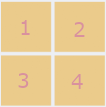
\includegraphics[width=0.3\textwidth,keepaspectratio]{images/numbering_board_2x2.PNG}
\end{figure}

\begin{comm}
    \label{ comm: indexing board game}
    מספור לוח שעובר על שורות ואז עמודות מלמעלה למטה כמו שמתואר באיור
    \ref{fig:numbering_board_2x2},
     היה שיטת המספור הקבוע בפרויקט זה עבור משחקים על לוח.
\end{comm}
ניקח דוגמה קצת יותר מסובכת
עבור גרף באיור
\ref{fig: change vector on graph}.
באיורים עלו נצבע בכחול צמתים שמצבם  
$1$
ובאדום 
צמתים שמצבם 
$0$.
בעזרת וקטור השינוי אפשר לתאר תוצאה של מספר לחיצות,
נעשה זאת בעזרת חיבור וקטור שינויים
וחיבור מצב הגרף.
התוצאה שנקבל 
תהיה הגרף המתקבל לאחר לחיצה של צמתים
הללו.
נדגים רעיון זה כאשר מצב של גרף מתואר באיור
\ref{fig:start graph presses}.
נניח שצומת 1 היא יחידה שדלוקה.
נרצה להראות איך הגרף יראה אם ילחצו על כפותרים 
$1, 3$.
וקטור שינוי של צומת 
$1$
הוא
\[
    t_1 = 
    \begin{bmatrix}
        1 \\
        0 \\
        1 \\
        1 \\
    \end{bmatrix}
\]
\[
    t_1 + t_3 = 
    \begin{bmatrix}
        1 \\
        0 \\
        1 \\
        1 \\
    \end{bmatrix}
    +
    \begin{bmatrix}
        1 \\
        1 \\
        1 \\
        1 \\
    \end{bmatrix}
    =
    \begin{bmatrix}
        0 \\
        1 \\
        0 \\
        0 \\
    \end{bmatrix}
\]
ומצב התחלתי שמתואר באיור נסמן ב
$S_0$
לכן מתקבל
\[
    S_0 + t_1 + t_3 = 
    \begin{bmatrix}
        1 \\
        0 \\
        0 \\
        0 \\
    \end{bmatrix}
    +
    \begin{bmatrix}
        0 \\
        1 \\
        0 \\
        0 \\
    \end{bmatrix}
    =
    \begin{bmatrix}
        1 \\
        1 \\
        0 \\
        0 \\
    \end{bmatrix}
\]
הגרף המתקבל לאחר חיבור אכן תואם לתוצאה המצופה
מתואר באיור 
\ref{fig:start graph presses solution}.

\begin{figure}[ht]
    \caption{
        דוגמה לתיאור וקטור שינוי במהלך משחק על גרף
        }
    \label{fig: change vector on graph}
    \centering
    \begin{subfigure}[b]{.4\linewidth}
        \caption{מצב של הגרף לפני לחיצה}
        \label{fig:start graph presses}
        % \unsethebrew
        \centering
        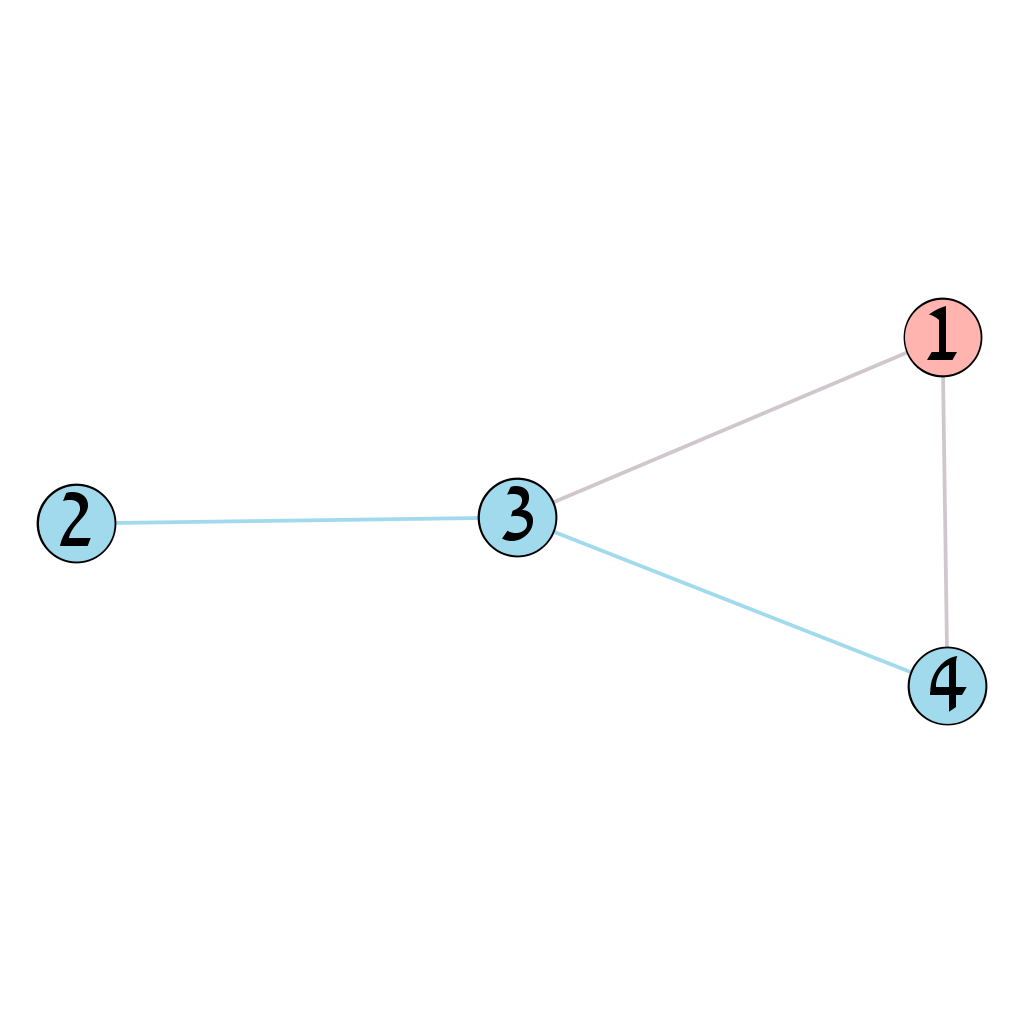
\includegraphics[width=.7\textwidth,keepaspectratio]{images/graph_presses.png}
    \end{subfigure}
    \begin{subfigure}[b]{.4\linewidth}
        \caption{מצב של הגרף לפני לחיצה}
        \label{fig:start graph presses solution}
        % \unsethebrew
        \centering
        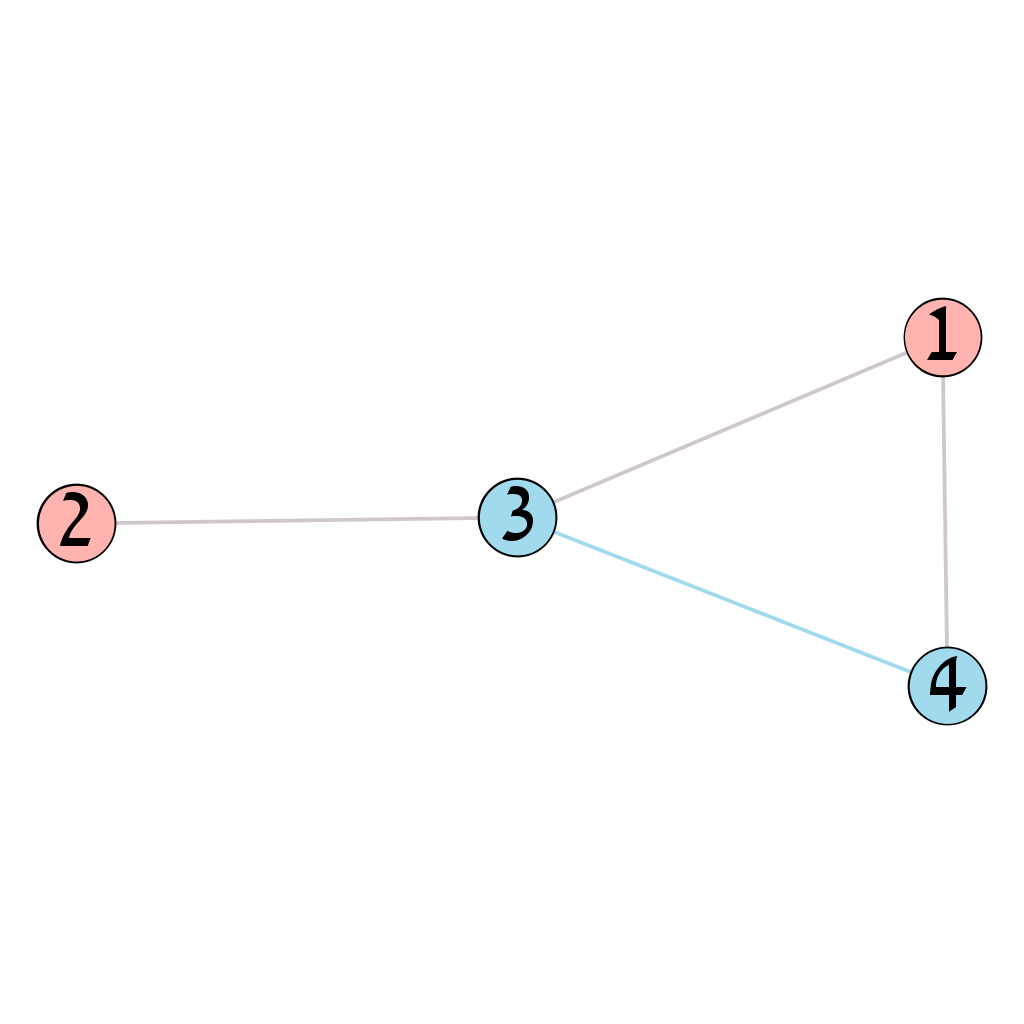
\includegraphics[width=.7\textwidth,keepaspectratio]{images/graph_presses_solve.png}
    \end{subfigure}
\end{figure}

\begin{comm}
    היות ווקטור שינוי שדה
    $\Zn$
    חיבור בין וקטורים הינו חיבור בין האינדקסים מודולו 
    $2$
    וכפל בסקלר
    הוא לכפול את כל ערכי וקטור בסקלר
    כאשר הסקלרים יכולים להיות
    $0$
    או 
    $1$
\end{comm}
\begin{comm}
    מספר זוגי של לחיצות אינו משנה את מצב הלוח
\end{comm}
היות 
ואנחנו עובדים על שדה מודולו 
$2$
$t_i + t_i = \vec{0}$.
\begin{comm}
    \label{comm: press is uneven presses}
    לא משנה כמה תלחץ על לחצן בודד הלחצן 
    יכול להעביר אותך לשני מצבים.
\end{comm}
מספר הלחיצות על אותו לחצן אינו משנה 
לחצן עכשיו 
לחוץ אם נלחץ מספר אי זוגי של פעמים 
כי מספר לחצות הזוגיות לא שינו את הלוח.
בנוסף זה מסביר את הסיבה למה כפל בסקלר שאנחנו מוכנים לקבל הוא הערכים 
$0,1$.
לכן בהמשך
הפתרון יתואר אם יש צורך ללחוץ בלחצן או לא,
לא תהיה התייחסות לכמות הלחיצות כי התוצאה מתקבלת רק תלויה בזוגיות של מספר הלחיצות.

\begin{comm}
    היות ומצב התחלתי הוא שכל הצמתים 
    במצב 
    $0$
    לכן,
    ניתן לתאר 
    את המצב עליו נעבור
    רק
    בעזרת צירוף לינארי של וקיטורי שינוי בלבד.
\end{comm}
היות ומצב התחלתי נסמן כרגע ב
$S_0$
הוא כולו וקטור האפס
מתקיים:
\begin{equation}
    \label{eq: sum change vectors}
    S_0 + \sumi{j} \vec{t_j} x_j=  \sumi{j}  \vec{t_j}x_j
\end{equation}
בעקבות כך ניתן לתאר את בעיית המשחק לצורה הבאה:
\begin{equation}
    \label{eq: lin eq for solving problem}
    \sumi{j} \vec{t_j} x_j = \vec{1}
\end{equation}
כאשר
$\vec{1}$
וקטור שכל ערכיו אחדים,
שזהו מצב הסופי של הגרף
ו
$n$
מספר הצמתים בגרף.
נשים לב 
שאם 
ידוע צירוף
$x = \begin{bmatrix}
    x_1, & x_2, & \cdots , x_n
\end{bmatrix}$
שמקיים את המשוואה 
\ref{eq: lin eq for solving problem}
קיבלנו פתרון של משחק על גרף.
כדי להגיע לפתרון על גרף נלחץ על הצמתים שמספורם 
שווה 
לאינדקסים 
שמקיימים
$x_j = 1$
בצירוף 
$x$.

בנוסחה
\ref{eq: sum change vectors}
קיימים מספר תכונות 
שנרצה לציין.
\begin{lemma}
    \label{lemma: order presses}
    סדר הלחיצות לא משנה את התוצאה הסופית
\end{lemma}
בגלל אסוציאטיביות של חיבור בשדה 
סדר לחיצות לא משנה.
\begin{lemma}
    \label{lemma: num presses}
    כמות האפשרויות לחיצה על לוח
    $m \times n$
    הוא 
    $2^{m \cdot n}$
\end{lemma}
לפי הערה 
\ref{comm: press is uneven presses}
כל לחצן יכול להיות בשתי מצבים 
והיות לפי
למה
\ref{lemma: order presses}
סדר הלחיצות לא משנה 
לכן ללוח
$m \times n$
מספר אפשרויות לחיצה 
$2^{m \cdot n}$.
כדי להבין את עוצמה של מספר מסדר שכזה נסתכל במשחק על לוח 
$6 \times 6$
כמות  אפשרויות לחיצה גדולה 
מכמות הסטנדרטית שמציגים מספר שלמים,
$4$
בתים
כלומר המספר הגדול ביותר שאפשר להציג  בעזרת 
$4$
בתים
הוא
$2^{32}-1$
המטרה של המחשה זה להדגיש כמה לא פרקטית לנסות לפתור בעזרת
ניסיון כל האופציות האפשריות.


מערכת משוואות 
שמתוארת בנוסחה
\ref{eq: lin eq for solving problem}
אפשר לתאר במספר צורות.
נפוצה מבניהם היא
בעזרת מטריצה כמו שמתואר 
בנוסחה 
\ref{eq: matrix eq for solving problem}.
\begin{equation*}
    \begin{bmatrix}
        t_1 & t_2 & \cdots & t_n
    \end{bmatrix}
    \begin{bmatrix}
        x_1 \\
        x_2 \\
        \cdots \\
        x_n \\
    \end{bmatrix}
    =
    \begin{bmatrix}
        1 \\
        1 \\
        1 \\
        1 \\
    \end{bmatrix}
\end{equation*}
\begin{equation}
    \label{eq: matrix eq for solving problem}
    \begin{bmatrix}
        t_{1,1} & t_{1,2} & \cdots & t_{1,n} \\
        t_{2,1} & t_{2,2} & \cdots & t_{2,n} \\
        \cdots & \cdots & \cdots & \cdots\\
        t_{i,j} & t_{i,2} & \cdots & t_{i,n} \\
        \cdots & \cdots & \cdots & \cdots\\
        t_{n,1} & t_{n,2} & \cdots & t_{n,n} \\
    \end{bmatrix}
    \begin{bmatrix}
        x_1 \\
        x_2 \\
        \cdots \\
        x_n \\
    \end{bmatrix}
    = 
    \begin{bmatrix}
        1 \\
        1 \\
        \cdots \\
        1 \\
    \end{bmatrix}
\end{equation}
נשים לב שלמטריצה
$A$
במשוואה
\ref{eq: matrix eq for solving problem}
מתקבל ש
$A_{i,j} = 1$
כאשר 
$i, j$
צמתים שהם שכנים או זהים
$i = j$.
\begin{definition}
    \label{def: neighbor matrix}
    מטריצה שמתארת את משחק 
    שקבלנו במשוואה
    \ref{eq: matrix eq for solving problem}
    תקראה מטריצת שכנויות של משחק.
\end{definition}
\begin{comm}
    \label{comm: symetic matrix}
    היות וכל צומת שכנה היא שכנה אחד לשני לכן במטריצה
    סימטרית
\end{comm}
דוגמה למטריצה  המתקבלת מגרף באיור 
\ref{fig:start graph presses solution}:
\[
    \begin{bmatrix}
        1 & 0 & 1 & 1\\
        0 & 0 & 1 & 0\\
        1 & 1 & 1 & 1\\
        1 & 0 & 1 & 1\\
    \end{bmatrix}
\]

\begin{definition}
    \label{ def: solution vector}
    תהי משחק ומערכת משוואת שמתארת אותו מצורה 
    \ref{eq: matrix eq for solving problem} 
    נגדיר את וקטור פתרון כצירוף הערכים מביאים לפתרון
    של מערכת המשוואות
    ונסמן אותו ב
    $\vec{x}$
\end{definition}
נזכיר שאם
$\vec{x}$
וקטור פתרון של המערכת 
ו
$x_i = 1$
אז המשמעות שכדי לפתור את המשחק
צריך ללחוץ על לחצן 
$i$.
בנוסף 
נזכיר שאתכן שהיו כמה פתרונות אפשריים.
\begin{definition}
    \label{def: standard solution}
    שיטת פתרון בעזרת יצירת  מטריצה שכנויות על ידי וקטור שינויים תקראה
    שיטה מציאת פתרון לפי מטריצת שכנויות.
\end{definition}
תוצאה דומה אפשר לראות בפרק מהספר
\cite{B2}.
מרגע שהצלחנו לתאר את הבעיה מערכת משוואות לינארית
על שדה
$\Zn$
מכן נוכל להיעזר בכלים של אלגברה לינארית כדי למצוא את הפתרון כמו מציאת פתרון בעזרת דירוג,
מציאת מטריצה פסאודו הפוכה וכולי. 
\begin{comm}
    \label{comm: for board too many variables}
    כמות תאים במטריצה שכנויות שצריך ללוח 
    ריבועי 
    $[n \times n]$
    הוא
    $n^4$.
\end{comm}
עבור לוח 
$[n \times n]$
כמות הלחצנים 
$n^2$
ולכן גודל המטריצה שתוארה במשוואה
\ref{eq: matrix eq for solving problem}
היא 
$[n^2 \times n^2]$
כמות הזיכרון שצריך כדי לשמור מטריצה ללוח ריבועי שאורך צלע הוא
$n$
דורש לשמור מטריצה עם 
$n^4$
ערכים
.

\subsection{שיטה למציאת פתרון לפי שורה העליונה}
הצגנו גישה פתרון
בעזרת מטריצת שכנויות, 
כפי שתיארנו
בהגדרה
\ref{def: standard solution}.
נרצה להראות שיטה נוספת למציאת פתרון.
שיטת הפתרון שנציג נובעת מהערה 
\ref{comm: for board too many variables}
שכמות המידע שצריך לשמור גדל בקצב 
$n^4$,
\\
כאשר
משחק הוא על לוח ריבועי ש
$n$
מייצג
כמות המשבצות לשורה.

המאמר 
\cite{B1}
מציג שיטה שמציאה של פתרון עם מערכת משוואות לינארית שונה ממערכת שהצגנו קודם.
אומנם המערכות שונות אבל שני המערכות המשוואות מובילות לאותם פתרונות.

מערכת המשואות המתקבלת בשיטה במאמר 
\cite{B1}
על לוח
$n \times n $
היא 
$n \times n $
כלומר,
יש 
$n^2$
ערכים במטריצה.
צמצום כמות הערכים שכזה יכולה להוביל לחישוב מהיר יותר וניצול טוב יותר של מידע.

בפרק זה נציג את הגישה שמתוארת 
\cite{B1}
נתאר כמה הבחנות שיסתמכו ששני הגישות שקולות ושגישה החדשה הינה רק אופטימיזציה
ספציפית לצורה של מטריצה הנתונה.
את הגישה החדשה ניקרא לאורך כל הפרק שיטה למציאת פתרון לפי שורה העליונה.
\begin{definition}
    \label{def: spanish way}
    שיטה למציאת פתרון לפי שורה העליונה, היא שיטה שמבוססת על עיקרון 
    שאם, ידוע איזה כפתורים צריכים להילחץ בשורה העליונה כדי להגיע לפתרון, אפשר לגלות את כל שאר הכפתורים שצריכים להילחץ 
    כמעט מידית.
\end{definition}
נתאר את 
שיטה למציאת פתרון לפי שורה העליונה
כל שלב שנעשה
על לוח 
$3 \times 3$.
נניח שאיור 
\ref{fig: 3 x 3 board indexed}
מתאר את הלוח הנתון כאשר המשבצות הינן הלחצנים ומספור זה אינדקסים 
הממספרים לפי
הערה 
\ref{ comm: indexing board game}.
שיטה למציאת פתרון לפי שורה העליונה
מתבסס על רעיון,
שפתרון של המשחק הוא סדרה של לחיצות על משבצות מסוימות. נשייך
 לכל משבצת משתנה שיכול לקבל שני ערכים: 
 $0$
  אם משבצת הזאת מופיעה בסדרת לחיצות של פתרון
 ו-
 $1$
 אם משבצת הזאת כן מופיעה בסדרת לחיצות של פתרון המשחק.
  מראש לא ידוע לנו
 האם משבצות של שורה ראשונה יופיעו בסדרה הזאת או לא. אז משתנים של משבצות בשורה ראשונה הם
 $x_1, x_2, x_3$.

\begin{figure}[ht]
    \caption{לוח 
    $3 \times 3$
    עם אינדקסים}
    \label{fig: 3 x 3 board indexed}
    % \unsethebrew
    \centering
    \[\begin{bmatrix}
        x_1 & x_2 & x_3 \\
        x_4 & x_5 & x_6 \\
        x_7 & x_8 & x_9 \\
    \end{bmatrix}    
    \]
\end{figure}

על מנת שהנורה במשבצת ראשונה בשורה ראשונה תהיה דולקת סכום משתנה שלה 
ומשתנים של משבצות שכנות במודולו
$2$ 
חייב להיות 
$1$. 
\begin{equation}
    \label{eq: cond eq}
    x_1 + x_2 + x_4 = 1  
\end{equation}
לכן משתנה 
במשבצת ראשונה בשורה שניה,
שסימנו במשתנה 
$x_4$
חייב להיות שווה ל
$x_1 + x_2 +1 $
כי 
\[
    x_1 + x_2 + x_4 = 1 \Rightarrow x_4 = x_1 + x_2 + 1  
\]
על מנת שהנורה במשבצת שנייה בשורה ראשונה
כלומר, 
$x_5$
מדוגמה
תהיה דולקת סכום 
משתנה שלה ומשתנים של משבצות שכנות במודולו
$2$ 
חייב להיות 
$1$.
לכן משתנה שחייבים לשייך למשבצת שנייה בשורה שניה חייב להיות
 $x_1+x_2+x_3+1$
 כי
 \[
     x_1 + x_2 + x_3 + x_5 = 1 \Rightarrow x_5 = x_1 + x_2 + x_3 +1
 \]
 באופן דומה מחשבים ערכי משתנים של שאר המשבצות בשורה שנייה ואחר כך
 על פי אותם שיקולים ערכי משתנים של משבצות בשורות הבאות. 
\begin{definition}
    \label{ def: depndeciy equation}
    המשוואה של סכום
    משתנים של משבצת  
    $i$
    וכל שכניה
    תקראה
    משוואת אילוצים על לחצן 
    $i$
\end{definition}
משוואה 
\ref{eq: cond eq}
הינה משוואת האילוצים שללחצן
$4$.
עבור משחק לוח
ריבועי באורך שורה 
$n$
שהלחצנים ממספרים לפי הערה
\ref{ comm: indexing board game}
ניתן לנסח בנוסחה פשוטה:
\begin{equation}
    \begin{english}
    \label{eq: depndeciy equation}
    x^*_{i - n} + x^*_{i - 1} + x^*_{i} + x^*_{i + 1} + x^*_{i + n} = 1
    \hspace{10pt}
    x^*_i =
    \begin{cases}
        x_i & \text{if } i \in [1,n^2]
        \\
        0 & \text{otherwise}
    \end{cases}
    \end{english}
\end{equation}


נשים לב שבעזרת גישה שתיארנו כרגע נוכל למלאה כל השורה שניה.
כל שורה תלויה בשורה מלפניך לכן כך נוכל למלאה את כל השורות 
כמו שמתואר באיור 
\ref{fig: 3 x 3 board fill intire board}.
נדגים מילוי משבצת
$7$
משורה שלישית לכן נצטרך ששורה
שניה חושבה.
נסתכל על משבצת מעל 
כלומר משבצת 
$4$
ונסתכל למה שווה משוואת האילוצים שלה:
\[ x_0 + x_3 + x_4 + x_6 = 1 \]
לכן 
\[ x_6 = 1 + x_0 + x_3 + x_4  \]
היות ושורה שניה מולאה וידוע שערך משבצות 
באותה שורה: 
\begin{align*}
    x_3 &= 1 + x_0 + x_1 \\
    x_4 &= 1 + x_0 + x_1 + x_2
\end{align*}
נציב ערכים אילו
\begin{align*}
    x_6 &= 1 + x_0 + (1 + x_0 + x_1) + (1 + x_0 + x_1 + x_2) \\
    x_6 &= 1 + x_0 + x_2
\end{align*}
\begin{figure}[ht]
    \caption{לוח 
    $3 \times 3$
    מלאה}
    \label{fig: 3 x 3 board fill intire board}
    % \unsethebrew
    \centering
    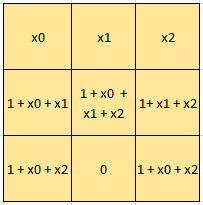
\includegraphics[width=.3\textwidth,height=.3\textheight,keepaspectratio]{images/3x3_fill_all.PNG}
\end{figure}
כדומה נעשה לשאר הערכים.
התוצאה מתקבלת מתוארת באיור 
\ref{fig: 3 x 3 board fill intire board}
נבחין שלאחר שמילאנו את כל הלוח כמו שמתואר באיור 
\ref{fig: 3 x 3 board fill intire board}.
לו הינו יודעים את את הערכים של  משתנים בשורה העליונה ביותר 
הינו כבר פותרים את המשחק.
על מנת ליצור מערכת משוואות
שתפתור את המשחק
מחבר המאמר
\cite{B1}
מוסיף לשורה האחרונה עוד שורה, שורה דמיונית ומחשב ערכי 
משתנים של המשבצות שלה לפי אותם שיקולים.

\begin{figure}[ht]
    \caption{לוח 
    $3 \times 3$
    מלאה
    כולל שורה וירטואלית
    }
    \label{fig: 3 x 3 board fill with virtual}
    % \unsethebrew
    \centering
    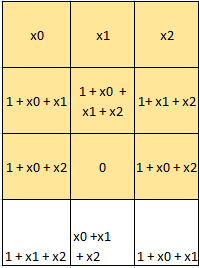
\includegraphics[width=.3\textwidth,height=.3\textheight,keepaspectratio]{images/3x3_fill_virtual.PNG}
\end{figure}

משום שזאת שורה דמיונית, 
בעצם אנחנו בפועל לא מדליקים אף נורה בה ערכי המשתנים של משבצות
שלה חייב להיות אפס.
כך נוצרת מערכת משוואות עם 
$n$
משוואות ו- 
$n$
משתנים וזה ההסבר שנתן מחבר המאמר. 
בהמשך כאשר נסביר קשר בין שיטה הזאת ושיטה הקודמת ניתן הסבר אחר. 
מערכת המשוואות המתקבלת עבור הדוגמה
$3 \times 3$.
\begin{figure}
    \caption{
        מערכת המשואות המתקבלת משיטה פתרון לפי שורה העליונה
        בלוח 
        $3 \times 3$
    }
    \label{fig: eq system for spanish method 3 x 3}
    
    \[\begin{cases}
        1+x_{1}+x_{2}=0\\
        x_0 + x_1 + x_2 = 0\\
        1 + x_0 + x_1 = 0
        \end{cases} \]
\end{figure}

שיטה שתיארנו ביצע מעבר על שורות אפשר היה לעשות בניה דומה גם לעמודות.
המאמר 
\cite{B1}
מתאר מספר רב של פתרונות  בלוחות ריבועים בגדלים שונה ואפילו על לוחות מלבניים.
האתגר המרכזי בשיטה הספרדית היא להצדיק אותה למה יש שורה וירטואלית
והאם יש קשר בין שני השיטות.
בשלב זה נתרכז להראות את הקשר בין שיטה הספרדית ושיטה שהצגנו בפרק הקודם.
\begin{theorem}
    מטריצה המיצג של מערכת המשוואות האילוצים היא מטריצת שכנויות
    \ref{eq: matrix eq for solving problem}.
\end{theorem}
משוואות האילוצים פורמלית היא לב השיטה הספרדית
מכיוון שהתקדמות בשורות מבוססת על המשוואות עלו.
אם נפרוס את משוואת האילוצים נקבל גם מערכת משוואת שפותרת את המשחק
אבל כמות המשואות הינה 
$n^2$.
נבחין שאם נציג אותם כמטריצה כאשר כל משוואת אילוצים מסודר לפי סדר הלחצנים נקבל את מטריצה שכנויות.

נדגים זאת על לוח 
$2 \times 2$
שמתואר באיור
\ref{fig: 2 x 2 board}.

\begin{figure}[ht]
    \caption{לוח 
    $2 \times 2$
    }
    \label{fig: 2 x 2 board}
    % \unsethebrew
    \centering
    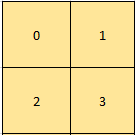
\includegraphics[width=.3\textwidth,height=.3\textheight,keepaspectratio]{images/2x2_board.PNG}
\end{figure}

וקטור השינויים:
\[
   t_0 = 
    \begin{bmatrix}
        1 \\
        1 \\
        1 \\
        0 \\
    \end{bmatrix},
    t_1 = 
    \begin{bmatrix}
        1 \\
        1 \\
        0 \\
        1 \\
    \end{bmatrix},
    t_2 = 
    \begin{bmatrix}
        1 \\
        0 \\
        1 \\
        1 \\
    \end{bmatrix},
    t_3 = 
    \begin{bmatrix}
        0 \\
        1 \\
        1 \\
        1 \\
    \end{bmatrix},
\]
לכן
מטריצת שכנויות נראת כך:
\[
    \begin{bmatrix}
        1 & 1 & 1 &0 \\
        1 & 1 & 0 & 1 \\
        1 & 0 & 1 & 1 \\
        0 & 1 & 1 & 1 \\
    \end{bmatrix},
\]
אם נסדר את המשוואות במערכת המשוואות לפי סדר 
האינדקסים של המשבצות נקבל את המערכת מהצורה
\begin{align*}
    x_0 + x_1 + x_2 &= 1\\
    x_0 + x_1 + x_3 &= 1\\
    x_0 + x_2 + x_3 &= 1\\
    x_1 + x_2 + x_3 &= 1
\end{align*}
אפשר בקלות לראות שאם נבנה את המטריצה המייצגת של המערכת נקבל מטריצה דומה למטריצת השכנויות.

תעלומה נוספת בשיטה הספרדית היא למה צריך שורה וירטואלי, למה ערכה 
שווה ל
$0$,
וכיצד באמת מתבצע צמצום כמות המשתנים ל
$n$
משתנים.
הסבר לתופעה זה
ניתן בעזרת תיאור שיטת מציאת פתרון לפי שורה העליונה רק שהפעם את
הפעולות במקום לעשות על טבלה שתיארה את הלוח נבצע על המטריצה שמתארת את מערכת המשוואות 
,
מטריצת השכנויות.
נראה את הפעולות שעושים בשיטה על אותה דוגמה 
על לוח 
$3 \times 3$

נשים לב ששיטה הספרדית מדרג את המטריצה מורחבת 
$[M | \vec{1}]$.

\begin{figure}
    \caption{
        מערכת משוואות מורחבת של משחק על לוח 
        $3 \times 3$
    }
    \label{fig: full matrix 3 x 3}
    \begin{english}
        \begin{center}
            \[
            \left[
            \begin{array}{ccccccccc|c}
                    1& 1& 0& 1& 0& 0& 0& 0& 0& 1 \\
                    1& 1& 1& 0& 1& 0& 0& 0& 0& 1 \\
                    0& 1& 1& 0& 0& 1& 0& 0& 0& 1 \\
                    1& 0& 0& 1& 1& 0& 1& 0& 0& 1 \\
                    0& 1& 0& 1& 1& 1& 0& 1& 0& 1 \\
                    0& 0& 1& 0& 1& 1& 0& 0& 1& 1 \\
                    0& 0& 0& 1& 0& 0& 1& 1& 0& 1 \\
                    0& 0& 0& 0& 1& 0& 1& 1& 1& 1 \\
                    0& 0& 0& 0& 0& 1& 0& 1& 1& 1 \\
            \end{array}
            \right]
            \]
        \end{center}
    \end{english}
\end{figure}


כדי לחשב את 
$x_4$
באיור
\ref{fig: 3 x 3 board indexed}
השתמשנו במשוואת האילוצים של 
משבצת 
$1$
שזה בדיוק תיאור
שורה הראשונה של 
מטריצה מורחבת 
בשורה הראשונה
שמתוארת
באיור 
\ref{fig: full matrix 3 x 3}.
\[
    x_1 + x_2 + x_4 = 1 \Rightarrow x_4 = x_1 + x_2 + x_3
\]
נבחין שלושת השורות הראשונות  
מאפשרות תיאור פשוט של המשתנים 
$x_4, x_5, x_6$.
אם ננסה לתאר 
את משתנה 
$x_7$
באותה שיטה 
נסתכל על שורה ה 
$4$
במטריצה 
וניראה שהיא תלויה ב
$x_4, x_5$
היות ואמרנו
שאפשר בקלות לתאר את משתנים עלו 
בעזרת שורות 
$1,2$
במטריצה לכן 
נעזר בשורות עלו כדי לתאר את 
$x_7$,
אופן שימוש בשורות עלו תהיה 
הפעלה פעולה שורות הבאה:
\begin{align*}
    r_4 \leftarrow r_4 + r_1
    \\
    r_4 \leftarrow r_4 + r_2
\end{align*}
שני פעולות שורות הללו הם שקולות לפעולה אלגברית הבאה
:
\begin{align*}
   (x_1 + x_4 + x_5 + x_7 + 1) + (x_1 + x_2 + x_4 + 1) = 0 \Rightarrow x_2 + x_5 + x_7 = 0
    \\
    (x_2 + x_5 + x_7) + (x_1 + x_2 + x_3 + x_5 + 1 ) = 0 \Rightarrow x_1 + x_3 + x_7 + 1 = 0
\end{align*}
ועכשיו קיבלנו תיאור 
של 
$x_7$
בעזרת המשתנים של שורה העליונה.
כך נמשיך באופן דומה לאופן שמילנו משבצות לפי שורה העליונה כך ניתן 
להמשיך ולמלאה את השורות במטריצה על ידי פעולות שורות המתבססות על 
חישוב קודם.
אחרי שנעבור על כל השורות בצורה שכזה נקבל את המטריצה:
\begin{figure}
    \caption{המטריצה לאחר פעולת שורות על כל שורות}
    \label{fig: matrix after spanish}
    \begin{english}
        \begin{center}
            \[
                \left[
                \begin{array}{ccccccccc|c}
                1& 1& 0& 1& 0& 0& 0& 0& 0& 1 \\
                1& 1& 1& 0& 1& 0& 0& 0& 0& 1 \\
                0& 1& 1& 0& 0& 1& 0& 0& 0& 1 \\
                1& 0& 1& 0& 0& 0& 1& 0& 0& 1\\
                0& 0& 0& 0& 0& 0& 0& 1& 0& 0\\
                1& 0& 1& 0& 0& 0& 0& 0& 1& 1\\
                0& 1& 1& 0& 0& 0& 0& 0& 0& 1\\
                1& 1& 1& 0& 0& 0& 0& 0& 0& 0\\
                1& 1& 0& 0& 0& 0& 0& 0& 0& 1\\
            \end{array}
            \right]
            \]
        \end{center}       
    \end{english}
\end{figure}
נשים לב שבמטריצה 
\ref{fig: matrix after spanish}
שלושת השורות התחתונות מתוארת אך ורק על 
ידי 
המשתנים 
$x_1, x_2, x_3$.
אם נתאר את שורות עלו כמערכת משוואות נקבל
את אותה מערכת משוואת של 
שיטה למציאת פתרון לפי שורה העליונה על לוח 
$3 \times 3$
שתיארנו במערכת המשוואות
\ref{fig: eq system for spanish method 3 x 3}.



\subsection{השוואה בין שתי השיטות למציאת פתרון}
לפי חישוב סיבוכיות
לדרג מטריצה 
כללית
בגודל 
$n^2 \times n^2$
זה 
$O(n^2 \cdot n^4) = O(n^6)$.

דירוג בעזרת שיטה הספרדית אומרת
שעל כל עמודה 
וקטור עמודה 
של מטריצת שכנויות
יש לכל יותר
$5$
ערכים ששווים 
$1$.
כל החוכמה בדירוג בשיטה הספרדית היא 
שפעולות השורות הם על משתנים שכבר דורגו
לכן 
כמות הפעולות שורות לא משתנה.
לכן דירוג שורה היה חיבור 
של עד כ
$5$
שורות
לכן הסיבוכיות 
$O(n^2 \cdot n^2) = O(n^4)$
.

לדרג את
$n$
משתנים  
הנותרים
הוא בסיבוכיות 
$O(n \cdot n^2) = O (n^3)$.

ננסה להראות זאת בפועל על ידי חישוב זמני חישוב.

\begin{figure}[ht]
    \caption{ 
    גרף מתאר ביצועים על לוח ריבועי גודל שורה מול זמן
    }
    \label{fig:prefofmance_diagram}
    % \unsethebrew
    \centering
    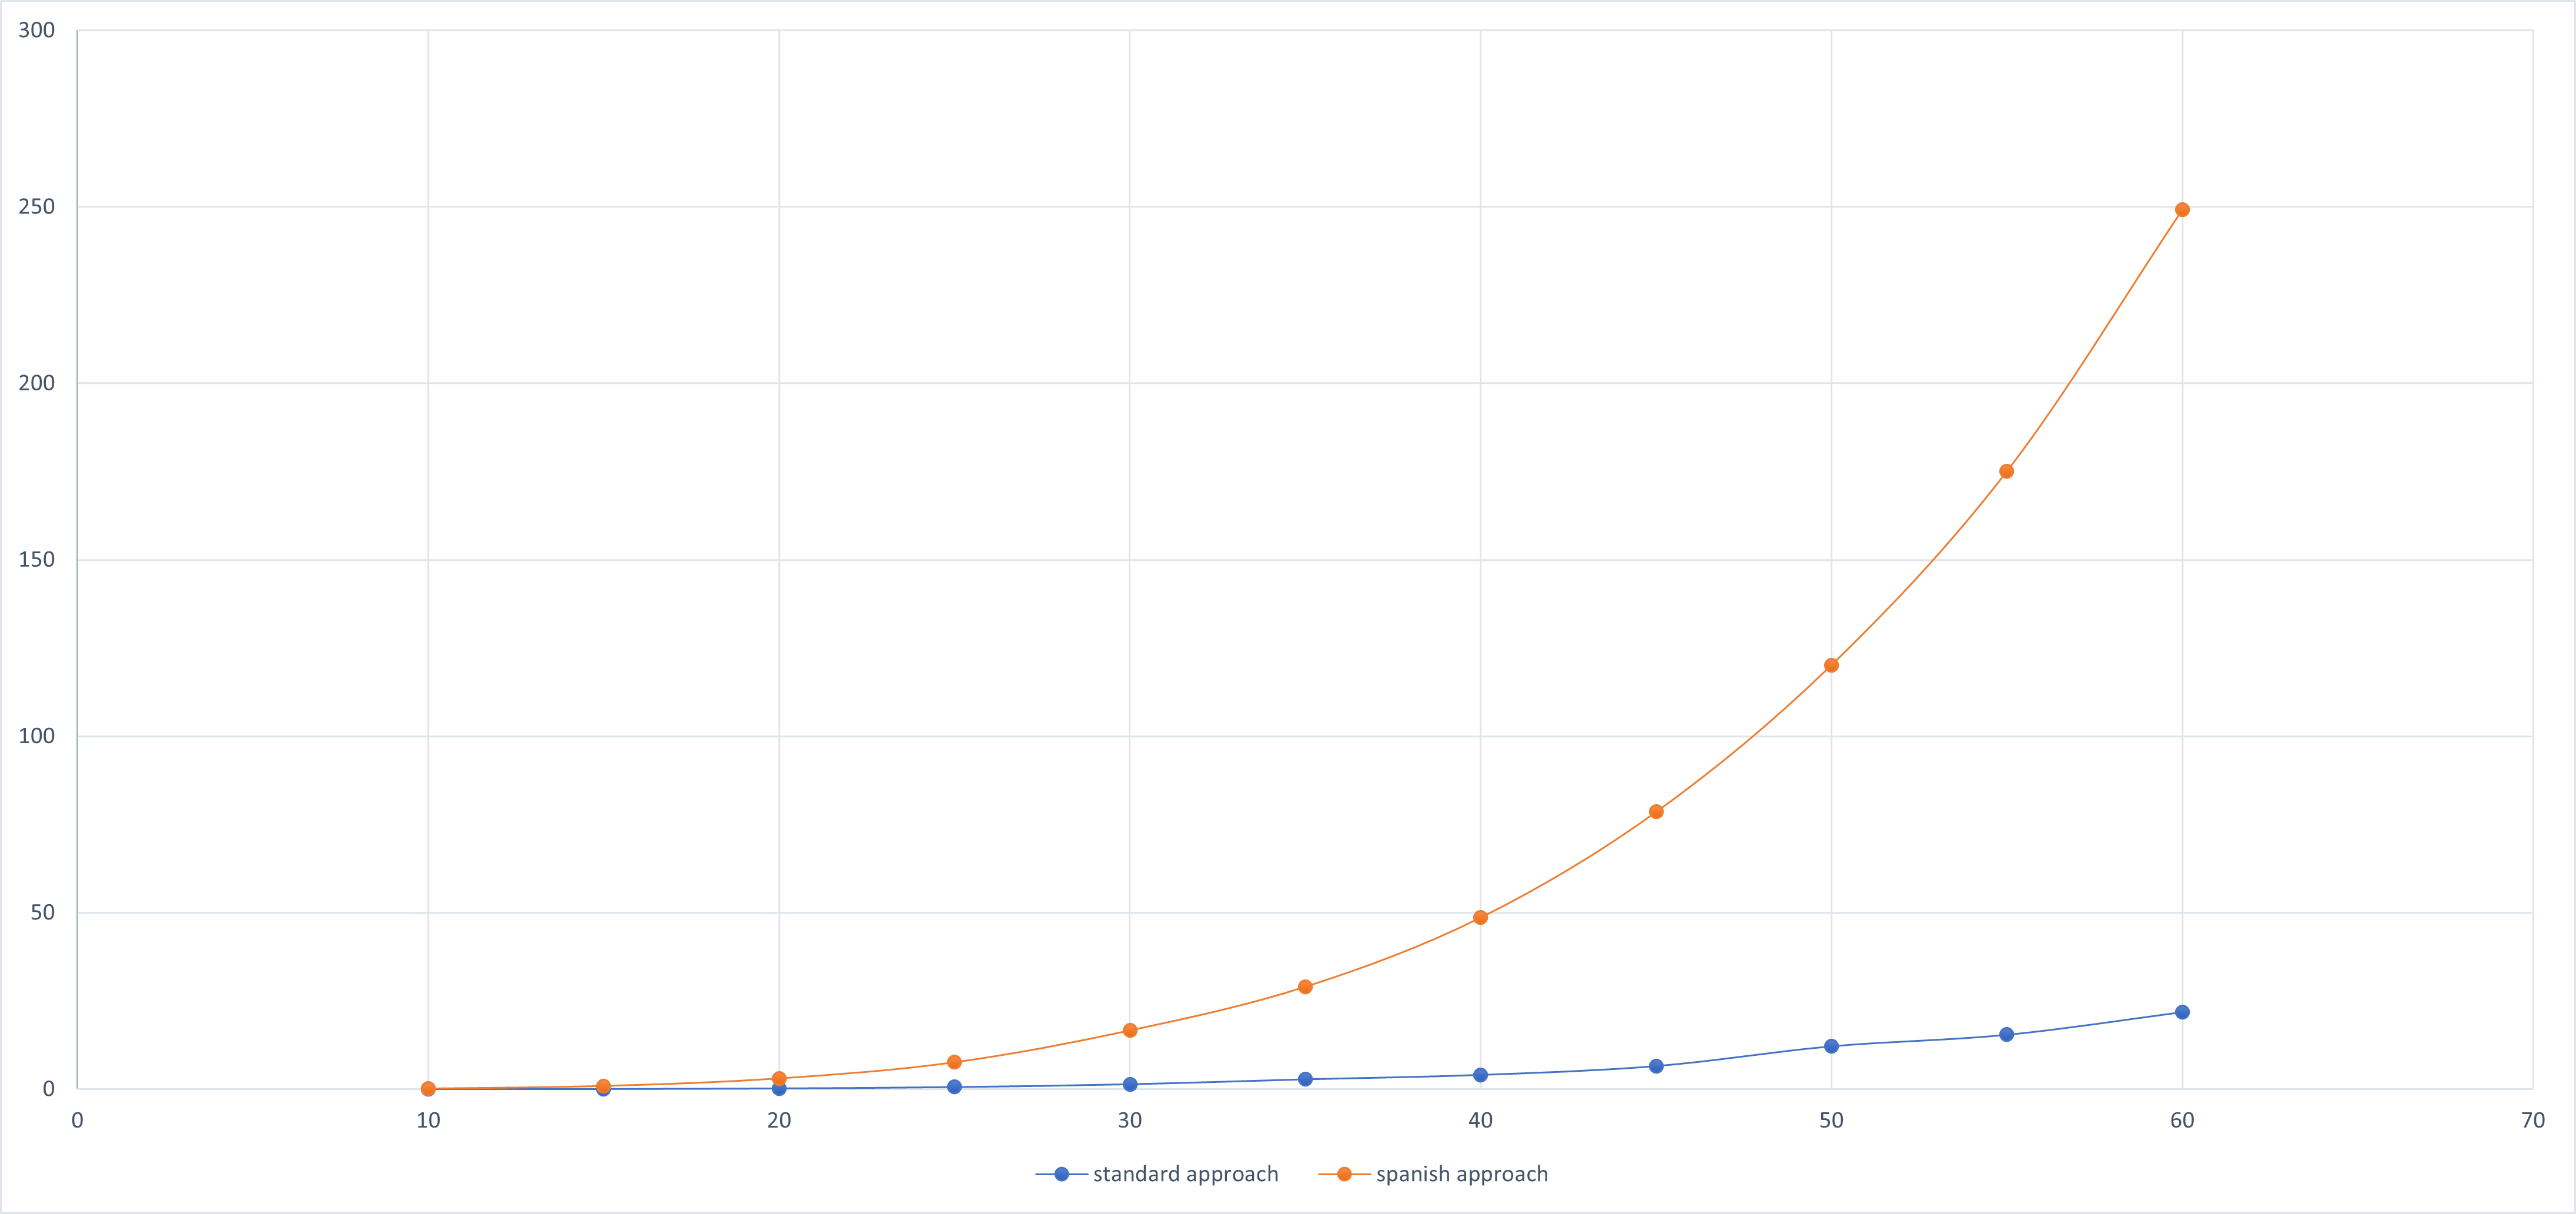
\includegraphics[width=\textwidth,height=\textheight,keepaspectratio]{images/benchmark.png}
\end{figure}
% \sethebrew

באיור 
\ref{fig:prefofmance_diagram}
אפשר לראות ביצועים
של שני האלגוריתמים ציר 
ה
$x$
גודל שורה של לוח המלבני
הרצנו על 
לוח בגדלים 
מ
$10$
עד 
$60$
משבצות.
ציר ה
$y$
זמן שלקח 
בשניות
\\
לפי התוצאות של איור 
\ref{fig:prefofmance_diagram}
ניראה 
שגישה הספרדית שבתאוריה יותר אופטימליות לוקחת יותר זמן.
אחת הסיבות לקח 
שפונקציה שפותרת מערכת משוואות הינה פונקציה של ספירה שנעזרתי וכנראה יש מימוש אופטימלי לפתרון הבעיה שאפילו 
ששיטה הספרדית מקטינה את כמות 
המשתנים היא אינה יכולה להתחרות במימוש אופטימלי שממשה בספריה.

\subsection{דיון לגבי משחק על גרף}
קיימים הרבה סיבות בהם תירצה להגדיר את הבעיה על מבנה כללי שכזה:

\begin{enumerate}
    \item 
    ככול שמבנה כללי יותר תאוריה שאתה מפתח מתאימה ליותר בעיות.
    \item 
    קיימת תאוריה רחבה שפותחה על גרפים ואתכן שנעזר בה.
    \item 
    מבליט את מהות הבעיה והגדרה הבסיסית ביותר של המשחק.
\end{enumerate}

ארצה להתייחס לנקודה אחרונה, תיאור הבעיה של משחק
כאוסף של כללים על גרף.
\\
הקשר בין המשחק עצמו לתיאור לגרפי כל כך מהותי
שבשלב מסוים של הפתרון נקבל את אחת הצורות לייצג גרפים וזאת על ידי מטריצת שכנויות.

\newpage
\section{הוכחת  קיום פתרון עבור כל גרף}
עד כה הסתכלנו על שני גישות שונות למציאת פתרון
אבל שאלה טבעית לשאול היא האם בכלל קיים פתרון למשחק על לוח כלשהו?
אחת הדרכים לענות על שאלה שכזה היא פשוט לקחת את הלוח ולפתור בעזרת 
דרכי הפתרון שהצגנו.
אחת הבעיות בגישה של לחפש פתרון על לוח כלשהו היא 
נניח ואנחנו רוצים לממש את המשחק האורות שמיצר לוחות אקראיים, היות ולא בהכרח ידוע אם קיים פתרון 
נצטרך לבדה שקיים פתרון על כל לוח בעזרת אלגוריתמים למציאת פתרון שלוקח זמן 
אתכן והלוח ללא פתרון נצטרך לחפש לוח אקראי אחר
מה שיגרום לתהליך יצירת משחק להיות איטי.
לכן, נרצה בשיטה מתמטית להוכיח לעבור איזה משחקים יש פתרון.
בנוסף שאלה נוספת שאפשר לשאול היא כמה פתרונות יש ללוח.
מספר הפתרונות של הלוח יכול להעיד האם הלוח יותר קל או קשה לשחקן שמנסה לפתור אותו
לבד ללא אלגוריתם.
בפרק זה נענה על השאלות הללו.

אחד המקומות ששאלה זה נשאלה היא בספר 
\cite{B3},
בעבודתנו נראה הוכחה קצת שונה בעזרת הכלים שפיתחנו.

\begin{definition}
    \label{def:inner_mul}
    נגדיר פעולה 
    בין שני וקטורים ב
    $\Zn$
    ניקרא לה מכפלה סקלרית
    תסומן 
    $x \cdot y$
    ונגדיר אותה כך:
    \\
    תהי 
    $\vec{x}, \vec{y} \in \Zn$
    אז 
    \[
        \vec{x} \cdot \vec{y} = 
        \begin{bmatrix}
            x_1 \\
            x_2 \\
            \cdots \\
            x_n \\
        \end{bmatrix}
        \cdot 
        \begin{bmatrix}
            y_1 \\
            y_2 \\
            \cdots \\
            y_n \\
        \end{bmatrix}
        = 
        x_1 y_1 + x_2 y_2 + \cdots x_n y_n
    \]
    כאשר 
    פעולת חיבור בין האיברים 
    הינה 
    חיבור מודולו
    $2$
\end{definition}

\begin{comm}
    \label{comm:not_really_inner_mul}
    המכפלה הסקלרית שהגדרנו ב
    \ref{def:inner_mul}
    אינה מכפלה פנימית,
    \\
    היות ותכונה 
    $<\vec{u},\vec{u}> = 0 \Leftrightarrow \vec{u} = \vec{0} $
    לא מתקיימת.
\end{comm}

דוגמה 
שמסבירה את הערה
\ref{comm:not_really_inner_mul}:

\[
    \begin{bmatrix}
    1 \\
    1 \\
    \end{bmatrix}    
    \cdot 
    \begin{bmatrix}
    1 \\
    1 \\
    \end{bmatrix} 
    = 1 + 1 = 0
\]

\begin{comm}
    וקטורים 
    $\vec{x}. \vec{y} \in \Zn $
    יקראו מאונכים אחד לשני נסמן זאת 
    $\vec{x} \perp  \vec{y}$
    אם המכפלה הסקלרית שהלם שווה 
    ל
    $0$
    $\vec{x} \cdot \vec{y} = 0$
\end{comm}

\begin{theorem}
    \label{the: Nul A and Col AT}
    תהי מטריצה 
    $A \in {Z_2}^{m \times n }$
    אז 
    $ColA^T \perp Nul A$
    $ColA \perp Nul A^T$
\end{theorem}

ידוע שתכונה זה מתקיימת 
ב
מטריצה 
$A \in R^{m \times n}$
ההוכחה 
ל
$ {Z_2}^{m \times n}$
זה
פרט ל
למכפלה הפנימית 
שדורשת 
לבצע על תוצר 
ב
$R^{m \times n}$
עוד 
מודלו 
$2$.
היות ותוצר של מכפלה פנימית הינו אפס גם לאחר מודלו 
$2$
היה 
$0$.

\begin{theorem}
    \label{thrm: clean game has solution}
    לכל משחק על גרף כאשר המצב התחלתי בו כל הנורות במצב 
    $0$
    \\
    קיים פתרון למשחק.
\end{theorem}

לפי 
שיטת פתרון סטנדרטית 
שהגדרנו
\ref{def: standard solution}
ניתן לתאר את פתרון המשחק על גרף בעזרת מטריצה
שכנויות לפי הגדרה 
\ref{def: neighbor matrix}.
\\
מטריצה שכנויות
נסמן ב
$A \in {Z_2}^{n \times n}$.

נזכיר כמה תכונות חשובות
\begin{enumerate}
    \item 
    מטריצה סימטרית לפי
    \ref{comm: symetic matrix}
    \item 
    $A$
    המטריצה הינה ריבועית.
    \item 
    האיברים על האלכסון
    מטריצה 
    $A$
    ערכם שווה ל
    $1$.
\end{enumerate}

כדי להראות שלמשחק יש פתרון 
צריך להראות שקיי פתרון למערכת

\[A \vec{x} = \vec{1} \]

במקרה ש 
$A$
מטריצה הפיכה אז קיים פתרון יחיד.
עבור המקרה שמטריצה אינה הפיכה 
כלומר 
$Nul A \neq \{ \vec{0}\}$
ניקח 
$\vec{x} \in Nul A$
כלומר 
$A\vec{x} = \vec{0} \\$
$\vec{x}^T A \vec{x} = \vec{x}^T\vec{0} = 0 \\$
נסמן 
$\vec{x} = [x_1, x_2, \cdots, x_n]^T$

\begin{multline}
    \label{eq: quadratic form}
        \vec{x}^T A \vec{x} = a_{1,1}x_1^2 + 2(a_{1,2} + a_{2,1})x_1x_2 + \cdots 2(a_{1,n} + a_{n,1})x_1x_n + \\
        + a_{2,2}x_2^2 +  2(a_{2,3} + a_{3,2})x_2x_3 + \cdots  + 2(a_{2,n} + a_{n,2})x_2x_n + \cdots
\end{multline}

היות ומטריצה סימטריות
$a_{i,j} = a_{j,i}$
לכן
מתקבל
\[a_{i,j} - a_{j,i} = a_{i,j} + \cdots + a_{j,i} = 1 \]
נזכיר כי תוצאות של פעולת חיבור וחיסור מודלו 
$2$
זהות.

לכן
את המשוואה 
\ref{eq: quadratic form}
אפשר לפשט ל
\[ \vec{x}^T A \vec{x} = a_{1,1}x_1^2 + a_{2,2} x_2^2 +  a_{n,n} x_n^2\]

הבחנה נוספת לערך 
$0$
או
$1$
$x^2 = x$
לכן פישוט נוסף למשוואה 
\ref{eq: quadratic form}
אפשרי:
\[ \vec{x}^T A \vec{x} = a_{1,1}x_1 + a_{2,2} x_2 +  a_{n,n} x_n\]

לכן קיבלנו 
$ \vec{x}^T A \vec{x} = 0$
שמתקיים:
\[a_{1,1}x_1 + a_{2,2} x_2 +  a_{n,n} x_n = 0\]

כלומר 
$\vec{1} \perp  \vec{x}$
כאשר 
$x \in Nul A$
לפי משפט 
\ref{the: Nul A and Col AT}
מתקבל 
$\vec{1} \in Col A^T$
היות ומטריצה סימטרית 
$A^T = A$
לכן
$\vec{1} \in Col A$
והוכחנו שלמערכת
$A\vec{x} = \vec{1}$
יש פתרון.

\subsection{מספר הפתרונות עבור כל גרף}
הוכחנו שלכל משחק על גרף שמתחל עם כל לחצנים במצב 
$0$
יש פתרון ניזכר שסדר לחיצות
אינו משנה את התוצאה על הלוח לכן אם נילחץ על הלחצנים בסדר כלשהו 
לפי פתרון נקבל גרף כולו דלוק.

השאלה  שנשאל בפרק זה מה אפשר לומר על מספר פתרונות מפיתוח שעשינו.
נציין קודם שניקרא לשני פתרונות שונים אם קיים לפחות לחצן אחד שמבדיל בין הפתרונות 
כלומר קיים לחצן ששייך לפתרון ראשון ולא שייך לפתרון שני כפי שציינו קודם סדר
לחיצות לא משנה את הפתרון.
לכן פתרון הינו קבוצה של לחצנים.
בנוסף נזכר לפי הערה
\ref{comm: press is uneven presses}
מספר אי זוגי של לחיצות נחשב ללחיצה לכן מספר הלחיצות על אותו לחצן לא משנה 
אלה רק זוגיות של מספר לחיצות 
לכן לכל לחצן יש רק שני מצבים שיכול להיות 
לחוץ 
או לא.
כרגע נראה שקיים כמה פתרונות לדוגמא 
איור
\ref{fig: clic 3 node graph game}
המתאר משחק על גרף בו הצמתים כבויים.
היות וגרף הינו קליקה לכן לחיצה בודדת על אחד הצמתים תדליק את כל הלחצנים.

קבלנו 
$G = \{\{v_1\}, \{v_2\}, \{v_3\} \}$
היא קבוצת של פתרונות.
כלומר כבר הראינו שיש מקרים בהם יש יותר מפתרון אחד.

\begin{figure}[ht]
    \caption{משחק על גרף}
    \label{fig: clic 3 node graph game} 
    % \unsethebrew
    \centering
    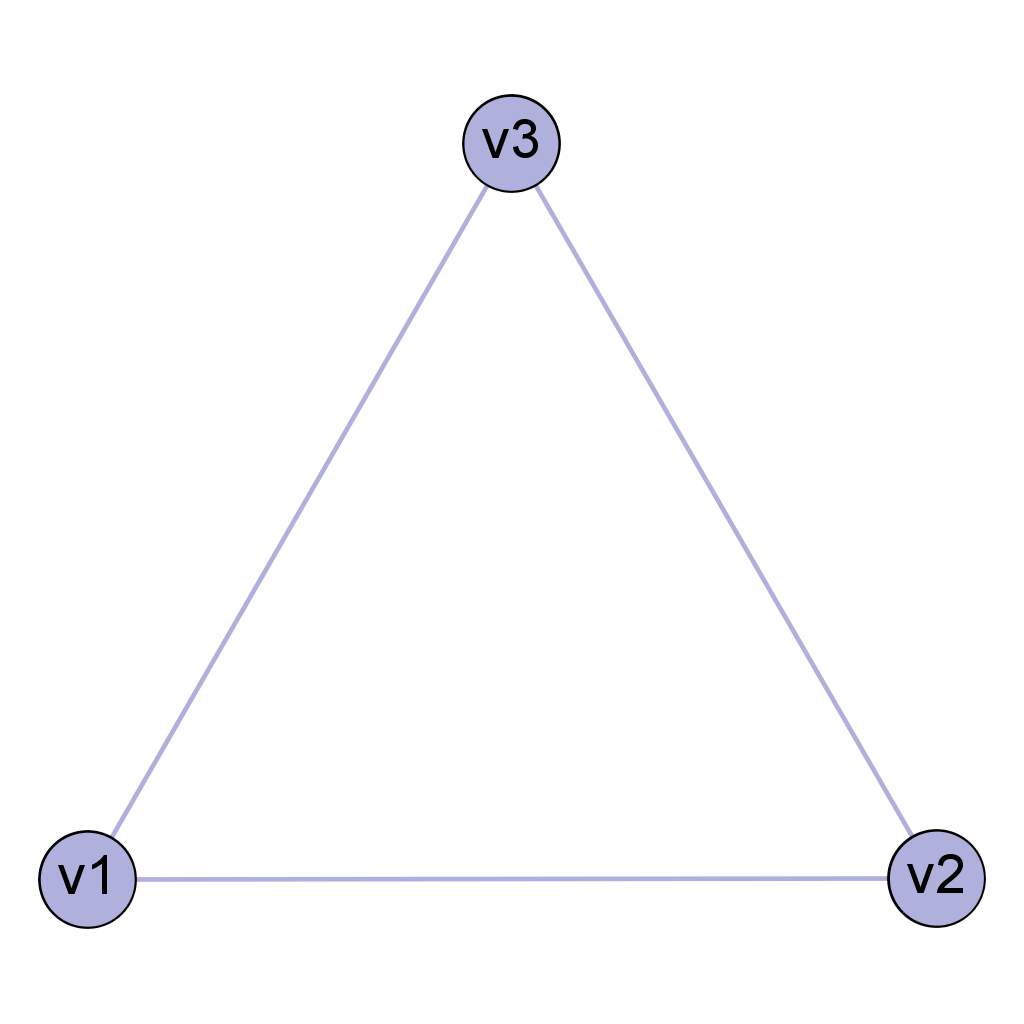
\includegraphics[width=.5\textwidth,height=.5\textheight,keepaspectratio]{images/clic_graph_3_node.png}
\end{figure}
% \sethebrew

שאלה טביעת שנובעת כשגילנו שיש היא כמה פתרונות יש למשחק מסוים.

\begin{theorem}
    מספר הפתרונות של משחק 
    שווה ל 
    $2^{k}$
    כאשר 
    $k$
    שווה לדרגת החופש של מטריצה
    $A$
    של פתרון הסטנדרטי
\end{theorem}

היות לכל משחק ניתן להגיר מטריצת שכנויות של משחק שהגדרנו 
ב
\ref{def: neighbor matrix}
ופתרונות של משחק וקטורים
$X$
של מערכת
$A X = \vec{1}$
כאשר 
$A$
מטריצת שכנויות.
ידוע שקיים פתרון למשחק ואם הוא משחק שמתחיל שמצב כל הנורות הוא
$0$
אז יש משפט 
\ref{thrm: clean game has solution}.
שמוכיח שקיים פתרון.

היות ומניחים שיש כמה פתרונות אפשר לתאר את כל פתרונות כ
$x = x_n + x_0$
כאשר 
$x_n \in Nul(A)$ ,
$x_0$ 
פתרון פרטי שידוע שקיים 
ו
$x$
כל פתרונות הכללים.

לכן מספר פתרונות כללים שווה למספר פתרונות במרחב האפס.
ידוע שמספר פתרונות במרחב האפס תלוי לדרגת החופש ולכן מספר הווקטורים שפורשים
את מרחב האפס שווה לדרגת החופש שנסמן ב
$k$.
כמות הווקטורים במרחב זה שווה לכל וקטורים שניתן ליצור בצירוף לינארי 

\[x = a_1 x_1 + a_1 x_1 + a_2 x_2 + \cdots + a_k x_k\]

כאשר הערכים של
$a_i \in Z_2$
לכן 
לכל מקדם יכול להיות
$2$
ערכים,
\\
לכן כל הקונבנציות האפשריות 
$2^k$
ששווה
לכמות הווקטורים 
במרחב האפס וכמות הפתרונות השונים של המשחק.

הבחנה נוספת ומעניינת שנרצה לציין היא בנושא חסם עליון לכמות הפתרונות.
חסם עליון טריוויאלי לכמות המקסימלית של פתרונות היא 
$2^n$
פתרונות כאשר
$n$
שווה למספר הלחצנים כלומר לא יכול להיות יותר פתרונות מאשר כמות הלחיצות השונות האפשריות במשחק.

\begin{comm}
    עבור משחק לוח מלבני
    בגודל 
    $m \times n$
    קיים לכל יותר 
    $2^k$
    כאשר 
    $k = \min{m,n}$
    פתרונות שונים
\end{comm}
הערה זה נכונה לפי גישה פתרון הספרדית
שהגדרנו
\ref{def: spanish way}
ניתן לתרגם את משחק ל
$k$
משוואות 
ש
$k$
יכול להיות מספר שורות או עמודות 
לכן ניקח את המספר הקטן יותר.


\section{פתרון מינימלי עבור לוחות מלבניים}
בפרק זה נציג פתרון לסוג מסוים של פתרונות שרצינו להציע. סוג זה של פתרונות 
מביאים רמז וניראה שמקלים את משחק. הקלה שכזאת על משחק אולי 
יכולה ליצור ביטחון לשחקנים חדשים וכמובן לאפיין תכונות לסוג של פתרון של כזה.

\begin{definition}
משחקים על לוח שקיים פתרון שלחצנים 
שינו את מצב רק פעם אחת.
למשחקים כאלו נקראה משחק מנמליים.
\end{definition}

באיור 
\ref{fig: min sol 2x3}
ניתן דוגמא לפתרון מינמלי 
בלוח 
$2 \times 3$.
כשלוחצים על לחצנים 
$2, 3$
על לוח כל נורות נדלקות ואף 
אחת מהם לא נכבה באף שלב של לחיצה.

\begin{figure}[ht]
    \caption{פתרון מינמלי של משחק}
    \label{fig: min sol 2x3}
    % \unsethebrew
    \centering
    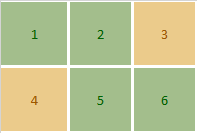
\includegraphics[width=.7\textwidth,height=.7\textheight,keepaspectratio]{images/min_sol_2x3.PNG}
\end{figure}
% \sethebrew

השאלה שנפתור בפרק זה לאיזה לוחות קיים פתרון מינמלי כאשר מצב התחלתי הוא שכל הנורות במצב
$0$.

\begin{definition}
    \label{def: dead zone}
    אזור מת זהו אוסף לחצנים בלוח
    שלחיצה עליהם 
    גורמת לחצן שכבר השתנה בעבר להשתנות שוב
\end{definition}

אזורים מתים על איור 
\ref{fig: min sol 2x3}
נראה שלאחר לחיצה על
לחצן
$2$
האזור מת שנוצר מלחיצה הינו
$\{0,1,2,4,5\}$

\begin{comm}
    אזור מת שנוצר מלחיצה 
    הוא כל הלחצנים במרחק לכל יותר 
    $2$
    משבצות מלחצן שנלחץ
    כאשר המרחק הוא מרחק מנהטן כלומר כל צדע למשבצת סמוכה למעלה למטה ימינה ושמאלה מגדילה את המרחק באחד
\end{comm}

\begin{figure}[ht]
    \caption{אזור מת שנוצר מלחצן באמצע הלוח}
    \label{fig: dead zone}
    % \unsethebrew
    \centering
    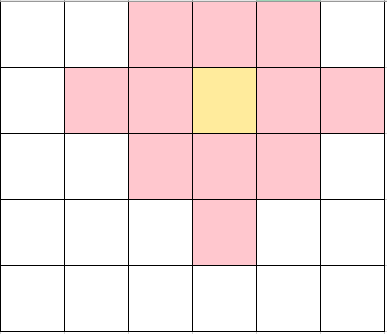
\includegraphics[width=.7\textwidth,height=.7\textheight,keepaspectratio]{images/dead_zone.PNG}
\end{figure}
% \sethebrew

באיור 
\ref{fig: dead zone}
אפשר לראות שאם נלחץ על לחצן בצהוב האזור המת הי האזור באדום כולל 
הלחצן עצמו.
תכונה זה כלי מרכזי בהוכחה במשפט הבאה

\begin{theorem}
    \label{thrm: bigger then 7x7 board no minimal solution}
    במשחק על לוח 
    $m \times n$
    שמתקיים
    $\min(m,n) >= 7$
    למשחק אין פתרון מינמלי
\end{theorem}

נניח ויש לנו לוח דו ממדי שמתואר כך נקודת התחלה בכיוון למטה 
"קומת ראשונה"
והולך כלפי מעלה לאינסוף 
ואינסוף לצד ימין וצד שמאל.
\\
נקרה לכל שורה אינסופית
קומה ונמספר אותם מאחת לאינסוף לכן קראנו לקומה נמוכה ביותר קומה ראשונה

נרצה למצוא פתרון מינמלי ללוח
וגישה לחיפוש הפתרון תהיה
להדליק שורה אחר שורה במלואה,
\\
היות ושורת אינסופיות נציעה אסטרטגיה להדלקת השורה וניראה את הקשיים שנפגוש.
\\
אם נרצה להדליק 
את כל קומה ראשנה רק על ידי לחצות 
בשורה ראשונה נקבל את הדפוס 
שאם לחצתי על לחצן מסוים חייב אני ללחוץ על לחצן
$3$
מימינו
כמו שמתואר באיור
\ref{fig: fill first stage only pressing first stage}
שמתאר לחצנים בירוק כלחצנים שנלחצו 
צהוב לחצנים שנדלקו ובאדום אזורים מתים שלא נדלקו.
באיור מוצג רק שתי לחיצות עוקבות של אסטרטגיה זה אבל כך נדליק את השורה הראשונה.

נשים לב באיור 
\ref{fig: fill first stage only pressing first stage}
על שני אזורים המתים הצמודים שלא נדלקו שצמודים אחד לשני כדי להדליק את שינהם
לא נוכל לעשות זאת ללא כיבוי לחצן שכבר נדלק.
זאת אומר שאסטרטגיה שכזאת
נפסלת עבור מילוי משחק שקומה שלו גדולה מ
$1$.

\begin{figure}[ht]
    \caption{מילוי קומה ראשונה על ידי לחיצות רק בקומה ראשונה}
    \label{fig: fill first stage only pressing first stage}
    % \unsethebrew
    \centering
    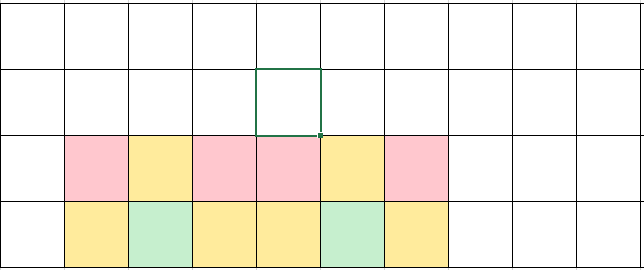
\includegraphics[width=.7\textwidth,height=.7\textheight,keepaspectratio]{images/first_stage_fill_only_first_stage_click.PNG}
\end{figure}
% \sethebrew

אסטרטגיה אחרת ויחידה למילוי קומה ראשונה הינה להדליק 
פעם לחצן בקומה ראשנה 
ופעם לחצן בקומה שניה צמודים.
היות ורק שני קומות ראשונות משנות את מצב הלחצנים בקומה ראשונה ולא קיים דפוסים נוספים
אפשריים למילוי שורה ראשונה בעזרת שני שורות עלו לכן עלו הן כל אסטרטגיות למילוי קומה ראשונה.

\begin{figure}[ht]
    \caption{מילוי קומה ראשונה}
    \label{fig: fill first stage second attempt}
    % \unsethebrew
    \centering
    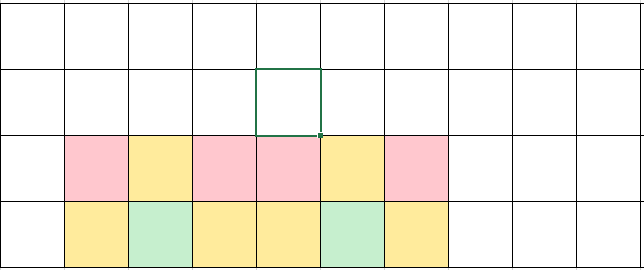
\includegraphics[width=.7\textwidth,height=.7\textheight,keepaspectratio]{images/first_stage_fill_only_first_stage_click.PNG}
\end{figure}
% \sethebrew

באיור 
\ref{fig: fill first stage second attempt}
אפשר לראות הדגמה קטנה של אסטרטגיה שכזה.

נרצה להראות אסטרטגיה שכזה מובילה לאזורים מתים שלא ניתן למלאות 
כל עוד רוצים שהפתרון היה מינימלי.
אם נסתכל באיור 
\ref{fig: fill first stage second attempt fails}
ניראה שאזורים המתים ששלשת
המשבצות הרצופות באדום לא ניתן היה למלאה אותם לכן צירוף כזה אין חוקי
כלומר הראינו שלמשחק כפי שהגדרנו לא קיים בכלל פתרונות מינימליים.

\begin{figure}[ht]
    \caption{מילוי קומה ראשונה}
    \label{fig: fill first stage second attempt fails}
    % \unsethebrew
    \centering
    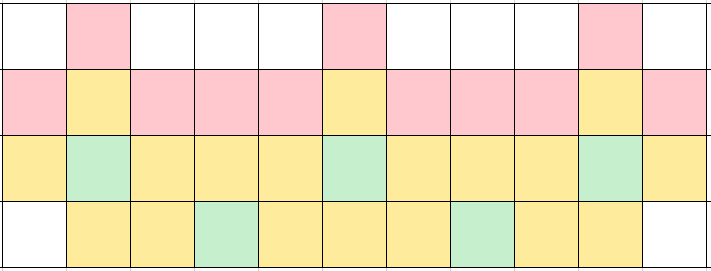
\includegraphics[width=.7\textwidth,height=.7\textheight,keepaspectratio]{images/first_stage_fill_only_first_stage_click_fail.PNG}
\end{figure}
% \sethebrew

בשלב זה נרצה להקטין את הרוחב ואורך כך שאם קיים 
משחק אופטימלי בלוח המוקטן אסטרטגיות המילוי קומה קומה היחידות 
שהיו חוקיות הן עלו שהצגנו.
נדע שהקטנה לא היו לה פתרונות אופטימליים אם היו משבצות סמוכות באזורים מתים.

נחזור ונסתכל על איור 
\ref{fig: fill first stage only pressing first stage}
נשים לב שלכל לוח שמספר המשבצות לרוחב גדול או שווה 
מ
$6$
שיטת המילוי שכזה תהיה לא חוקית כי היו 
$2$
משבצות סמוכות שבאזורים לא חוקיים.
ובאיור 
\ref{fig: fill first stage second attempt fails}
ניראה
שלרוחב גדול או שווה 
מ
$5$
היות ובניה
של קומה ראשונה מסתמכת על זה שיש 
$7$
משבצות ניקח ליתר ביטחון 
$7$
משבצות ולכן באסטרטגיה זה לא היה פתרון מינמלי.

קיבלנו שאפשר להקטין את הלוח לרוחב של
$7$
משבצות 
ועדיין לא היה פתרון  מינמלי. 

את אותם טענות אפשר היה לבנות לא רק להגביל את רוחב ל
$7$
משבצות עלה גם לגובה.
לכן לסיכום קיבלנו 
במשחק על לוח 
שאורך או רוחב גדולים או שווים מ
$7$
אז
למשחק אין פתרון מינמלי
והוכחנו את הטענה.


\subsection{הלוח הגדול ביותר בעל פתרון מינמלי}
טענה 
\ref{thrm: bigger then 7x7 board no minimal solution} 
מגבילה מאד את המשחקים שיש להם פתרון מינמלי ובשיטת הפתרון שהצגנו
אחד המסקנות המתקבלות שאם יש שלוש קומות או יותר מתחילה
להיות בעיתיות בגישת מילוי השורות.
אפשר להבחין בתופעה זה היות וקיים פתרון מינמלי למשחק 
$2 \times m$
כאשר 
$m$
הוא אי זוגי
האסטרטגיה השנייה מאפשרת מילוי קומות ולקבל פתרון מינמלי
נדגים זאת על באיור 
\ref{fig: 2x9 have min sol}

\begin{figure}[ht]
    \caption{פתרון ללוח 
    $2 \times 9$}
    \label{fig: 2x9 have min sol}
    % \unsethebrew
    \centering
    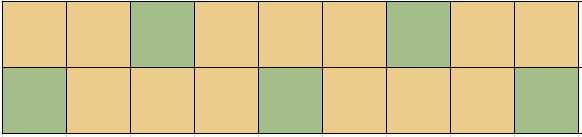
\includegraphics[width=.7\textwidth,height=.7\textheight,keepaspectratio]{images/2xm_sol.PNG}
\end{figure}
% \sethebrew

לאחר שהבנו שלוחות בגודל 
$2 \times m$
כאשר 
$m$
אי זוגי 
קיים פתרון מינמלי נשאל מהו הלוח 
הגדול ביותר
בעל פתרון מינמלי כאשר 
הלוח אורך ורוחב גדולים מ
$2$.

לפי טענה 
\ref{thrm: bigger then 7x7 board no minimal solution} 
אין טעם לבדוק לוחות שעמודות ושורות גדולים מ
$7$
ומבניית ההוכחה 
אמרנו שאם 
הגדול של עמודות או שורות לא קטן
מ
$3$
כלומר נותר לבדוק לוחות שממד שלהם 
$m \times n$
שייכים לקבוצה
$\{ (m,n) : 2 < m,n <7 \}$.

אפשר לנסות ולחפש פתרון ידנית
או לעבור על כל הפתרונות של משחק רגיל ולבדוק עם יש מבניהם פתרון 
מינמלי.
נציעה דרך אחרת לחפש פתרון 
מינמלי
והיא בעזרת להשתמש באותה מטריצה שכנויות כפי שהגדרנו רק להגדיר 
את זה שהיא על חוג 
$\mathbb{Z}$.
בעזרת שימוש בחוג 
$\mathbb{Z}$
מאלצים את שפתרונות המתקבלים
שידליקו כל נורות אך ורק פעם אחת,
זאת מתקיים בעקבות 
משוואות האילוצים שהגדרנו ב
\ref{ def: depndeciy equation}
שמאלצות את הסכום להיות שווה לאחד
,
אם נסתכל על נוסחה של משוואת האילוצים הכללים 
נוסחה
\ref{eq: depndeciy equation}
היות וחיבור על השלמים לכן 
מאולצים במשוואה זה שהיה לחצן בודד לחוץ 
לכן פתרון מערכת המשוואות מתאר פתרון 
מינמלי של משחק.
התיאוריה שפיתחנו באלגברה לינארית הייתה תקפה לשדות 
אבל כלי תכנות שהשתמשנו
בעבודה זה יודע לפתור גם על חוג של השלמים 
והסמכנו על הכלי כדי לבדוק את המקרים
שממדים שייכם לקבוצה 
$\{ (m,n) : 2 < m,n <7 \}$
וקיבלנו שהלוח
היחיד בקבוצת הממדים העלו שיש לו פתרון מינמלי 
הוא
לוח 
$4 \times 4$
ופתרון מתואר באיור 
\ref{fig:4x4_have_min_sol}

\begin{figure}[ht]
    \caption{פתרון ללוח 
    $4 \times 4$}
    \label{fig:4x4_have_min_sol}
    % \unsethebrew
    \centering
    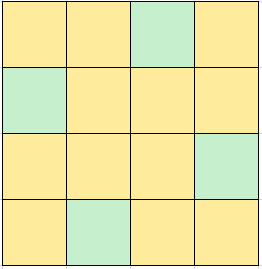
\includegraphics[width=.5\textwidth,height=.5\textheight,keepaspectratio]{images/4x4_min_sol.PNG}
\end{figure}
% \sethebrew

\newpage
\section{נספחים}
מימוש של הפרויקט בוצע על ידי 
שפת תוכנה 
{Python}
עם הכלי 
{Sage}.

% \unsethebrew
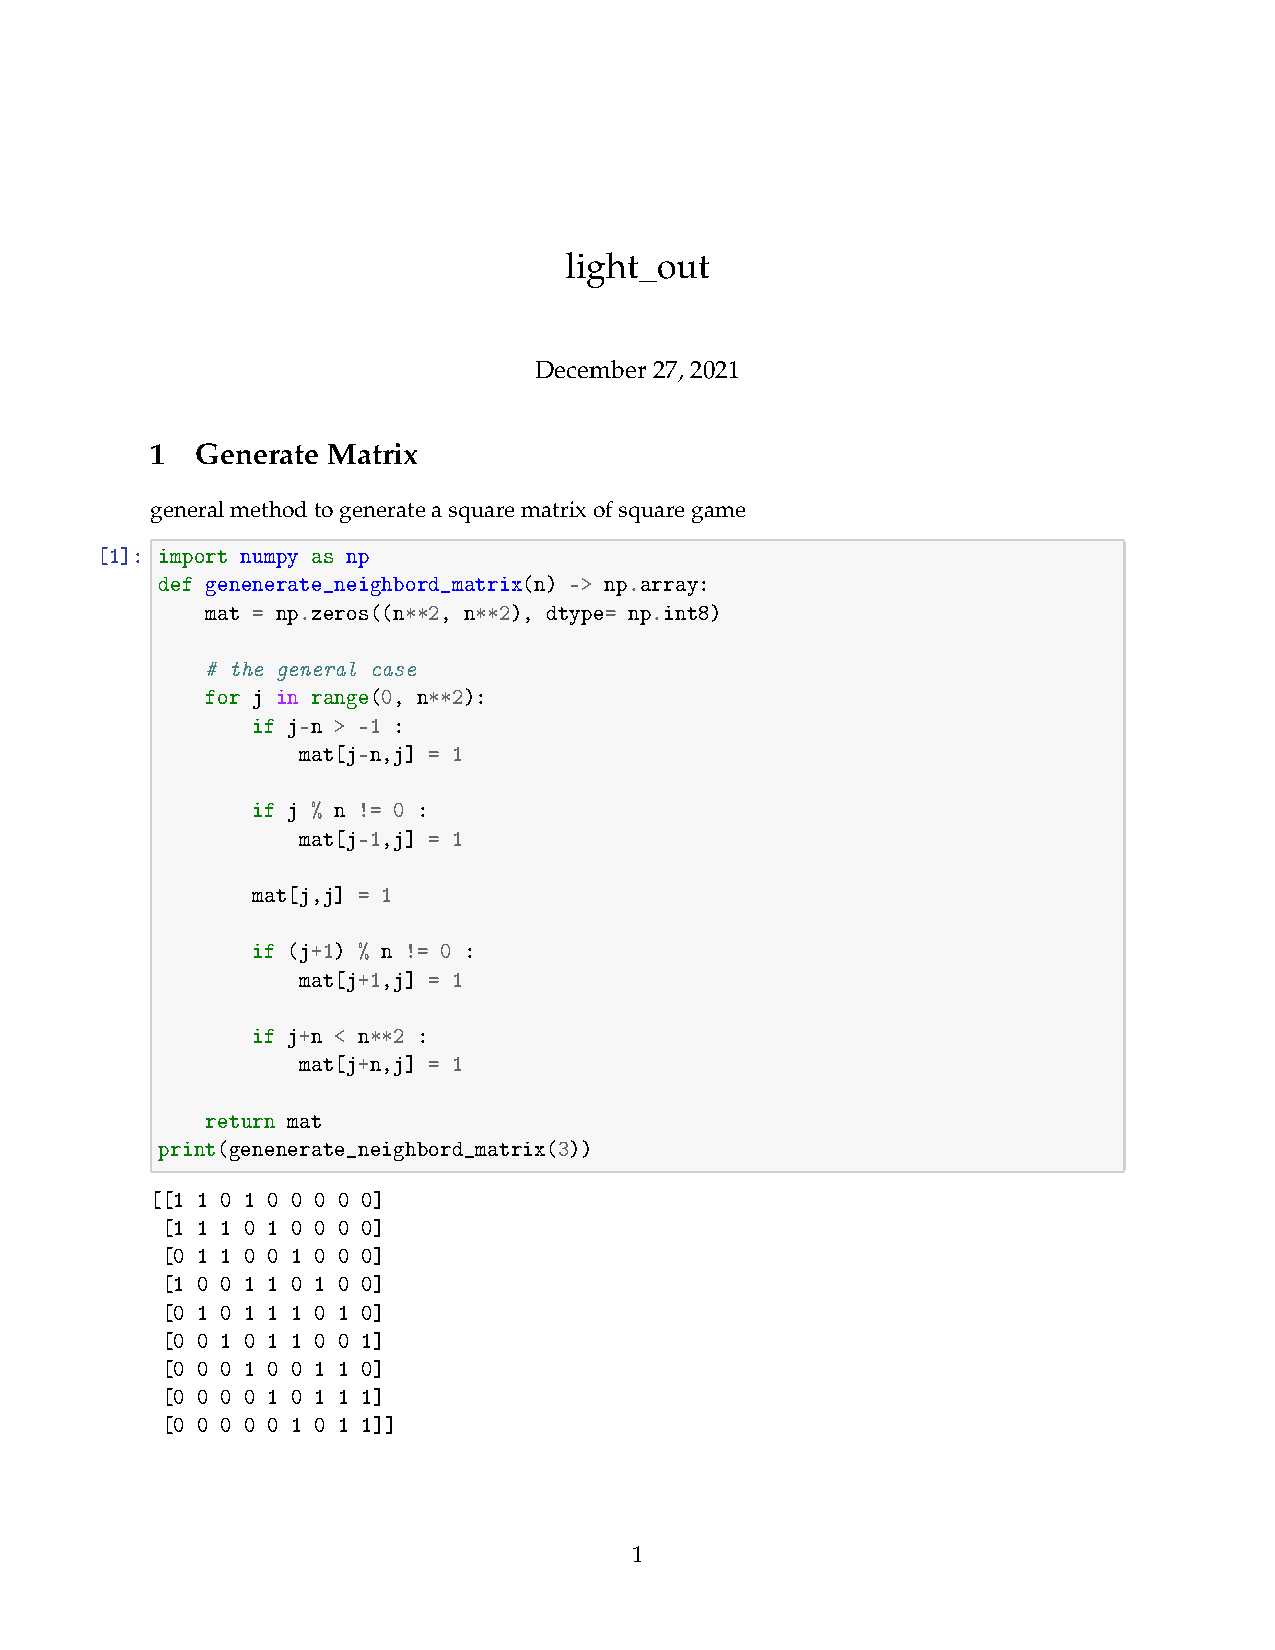
\includepdf[pages=-]{light_out_jupyter.pdf}
% \sethebrew
%----------------------------------------------------------------------------------------
%   רשימת מקורות
%----------------------------------------------------------------------------------------
\newpage
\begin{thebibliography}{99}
% \unsethebrew
\begin{english}
\bibitem{B1}
Rafael Losada
Translated from Spanish by Ángeles Vallejo,
\emph{
    ALL LIGHTS AND LIGHTS OUT,
}
SUMA magazine’s 
\bibitem{B2}
Jamie Mulholland
\emph{
    Permutation Puzzles
}
Lecture 24: Light out Puzzle , SFU faculty of science department of mathematic
\end{english}
\bibitem{B3}
אברהם ברמן, בן-ציון קון, 
\emph{
אלגברה ליניארית, תיאוריה ותרגילים
}
, הוצאת בק, חיפה, 1999.
\end{thebibliography}

\end{document} 
